\documentclass[12pt, a4paper, openany]{extarticle}
\usepackage{mystyle}
\selectlanguage{russian}

\begin{document}
\part*{Лабораторная работа №2\\
Получение конструктивной постоянной двигателя}

\section{Методические рекомендации}
\hspace*{\parindent}До начала работы студент должен выполнить предыдущую лабораторную этого цикла.
Также необходимо знание основ электродинамики.

\section{Теоретические сведения}
\hspace*{\parindent}В~данной лабораторной работе на примере двигателя EV3 мы продолжим изучение строения и принципов функционирования электродвигателя постоянного тока и рассмотрим протекающие в нем электродинамические процессы.

\paragraph*{Принцип работы и устройство двигателя}$\phantom{-}$\\
\hspace*{\parindent}Как известно, при внесении проводников с током в магнитное поле на них начинает действовать определенная сила, носящая имя \textit{силы Ампера}. 
Очевидно, что, если проводник оказывается никак не закрепленным, она вызывает его движение. 
Данное физическое явление и лежит в основе принципов работы любого электродвигателя. 
Это, естественно, отражается на их строении.

В~двигателях постоянного тока, подобных тому, который лежит в основе мотора EV3, роль упомянутого проводника играют размещаемые на роторе катушки (см.~рис.~\ref{rotor_in_life} или рис.~1 лабораторной работы №1). 
Именно в них мы создаем ток, подавая напряжение <<на двигатель>>. 
Других проводников в них нет. 
Магнитное поле, окружающее ротор, создается находящимися на статоре постоянными магнитами. 

Чтобы понять, как конструкции такого типа работают, рассмотрим простейшую модель двигателя. 
Ротор в ней будет представлен обычным прямоугольным контуром с током (см.~рис.~\ref{rotor_in_model}; на нем также изображено направление тока для случая, когда верхний контакт контура подключен <<к плюсу>>, а нижний~--- <<к минусу>>, и обозначения для длин его сторон), а статор~--- двумя постоянными магнитами (см. рис.~\ref{stator_in_model}; пунктирной линией на нем показана область, в которой вращается ротор, а пурпурными векторами~--- направление индукции $\vec{B}$ магнитного поля\footnote{Для простоты и наглядности следующих рассуждений мы будем считать, что магнитное поле нашего статора однородное и имеет конфигурацию, показанную на рис.~\ref{stator_in_model}.}). 

\begin{figure}[h]
	\begin{center}
		\begin{minipage}[h]{0.40\linewidth}
			\centering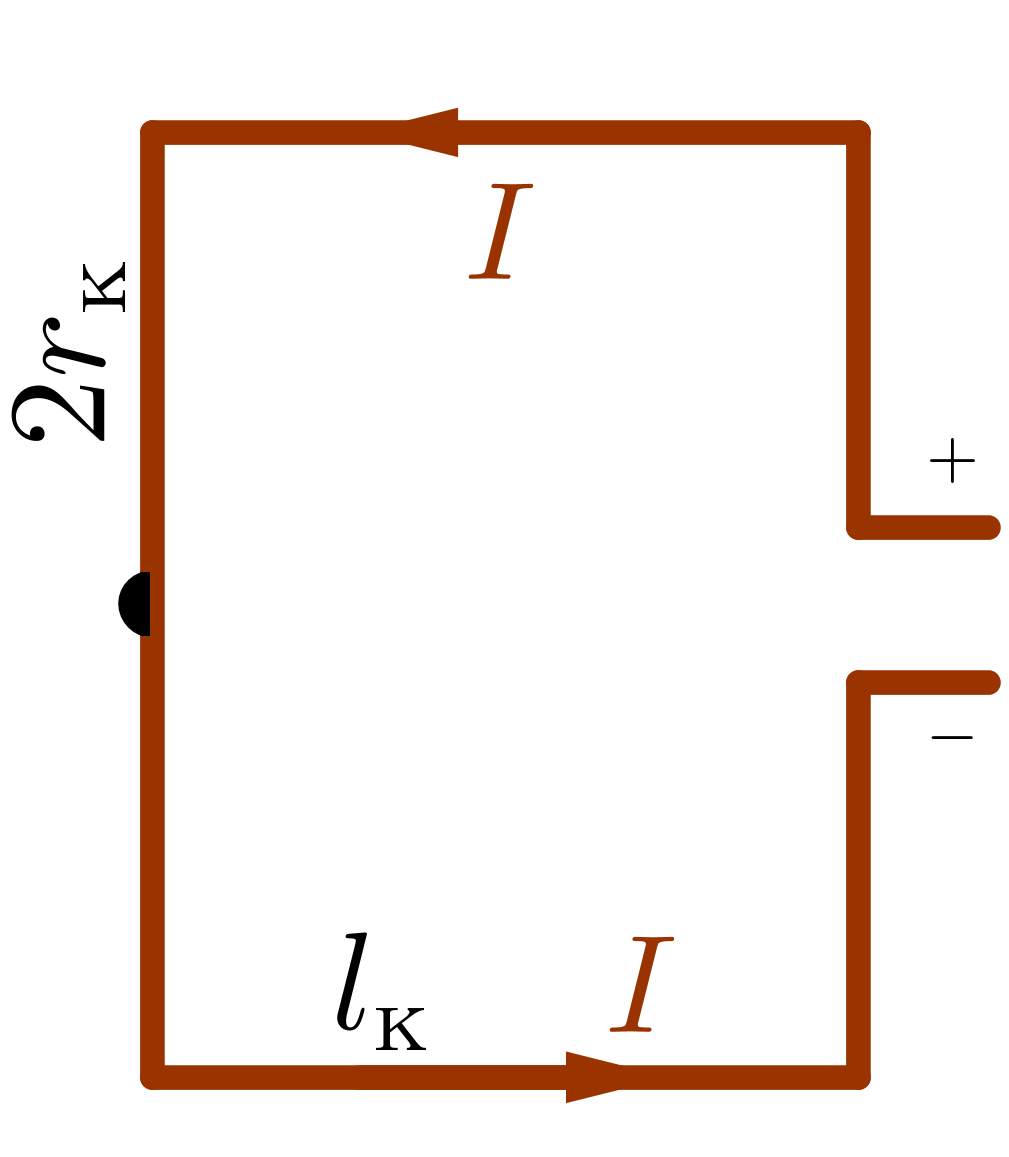
\includegraphics[height=4 cm]{pics/rotor_in_model.png}
			\caption{Модельный ротор.}
			\label{rotor_in_model} 
		\end{minipage}
		\hfill 
		\begin{minipage}[h]{0.59\linewidth}
			\centering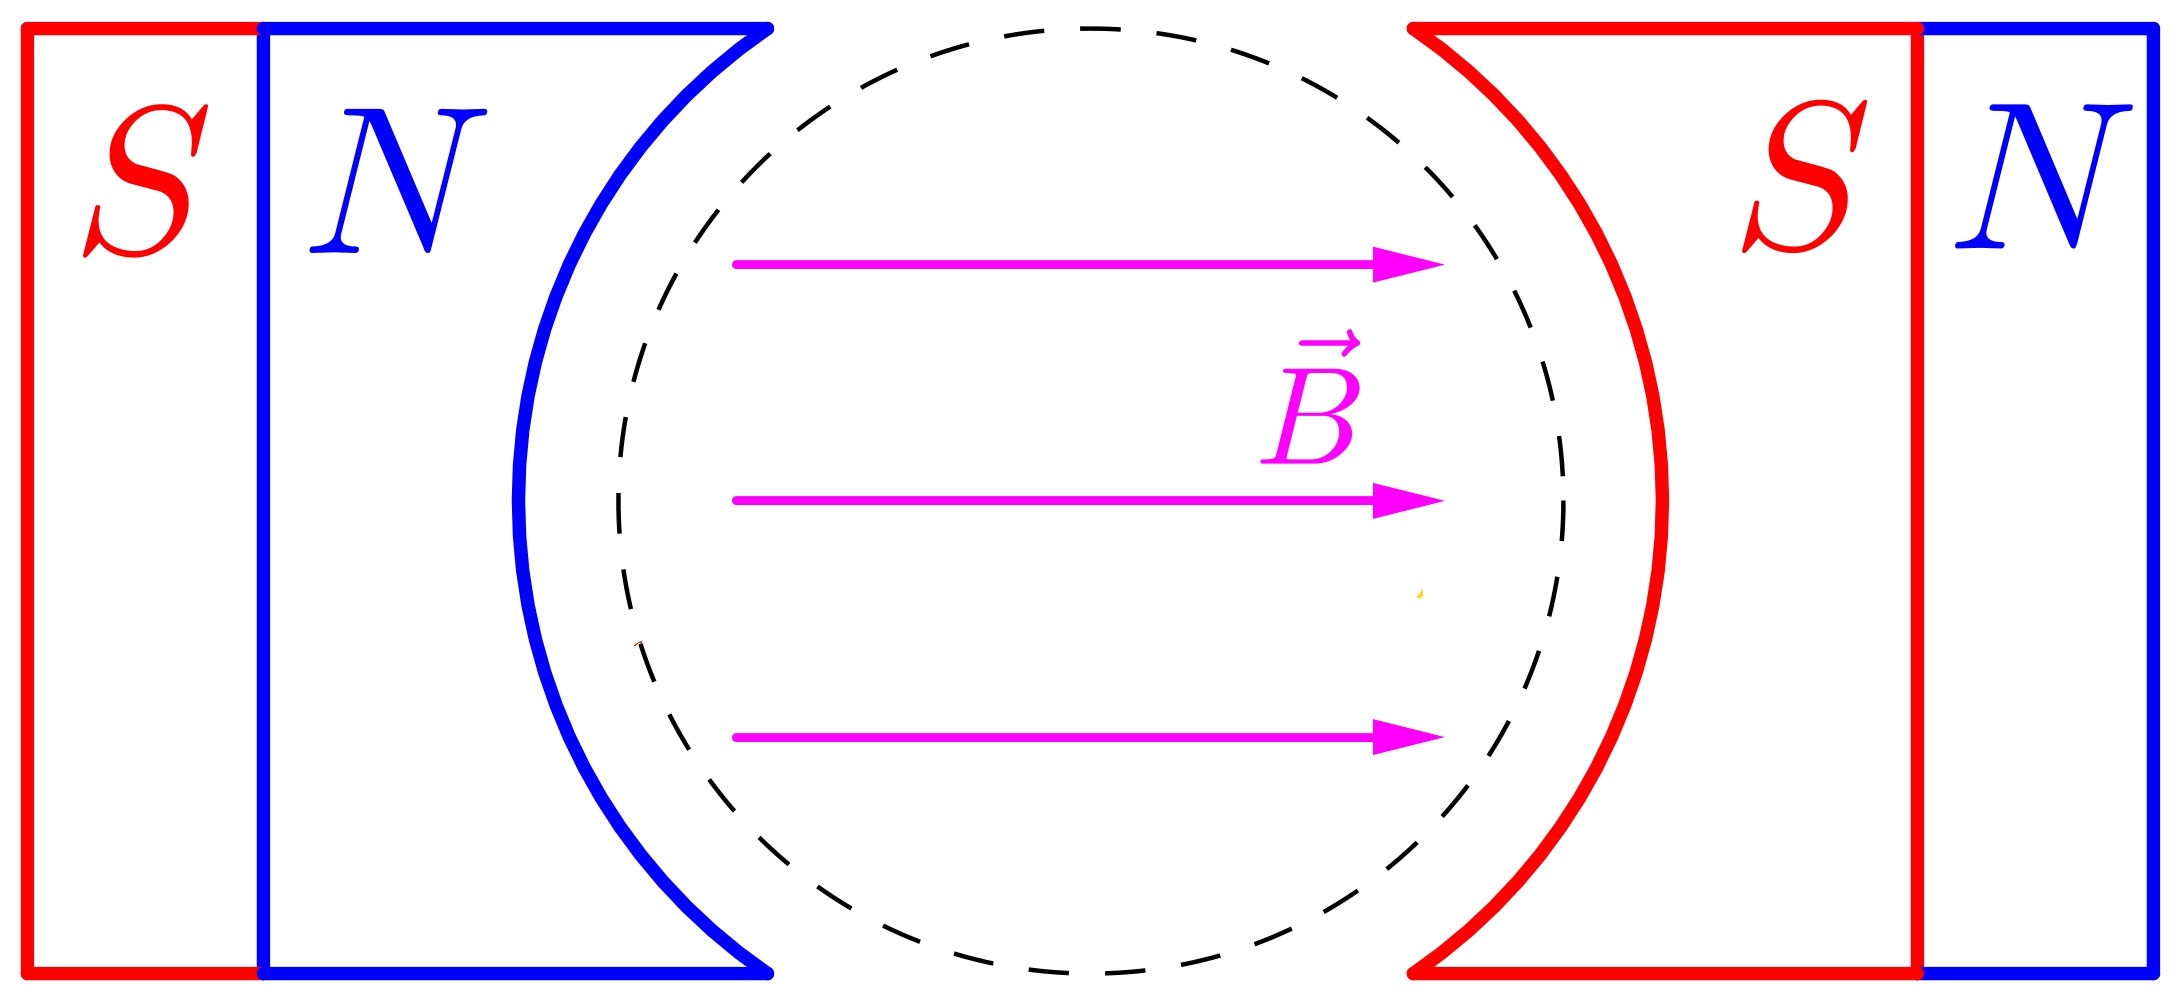
\includegraphics[height=4 cm]{pics/stator_2.png}
			\caption{Модельный статор.}
			\label{stator_in_model}
		\end{minipage}
	\end{center}
\end{figure}

Предположим, что в начальный момент времени ротор двигателя-модели занимал положение, показанное на рис.~\ref{1_phase} (плоскость контура ротора перпендикулярна плоскости рисунка). 
Тогда при указанном направлении тока и с учетом направления вектора $\vec{B}$ имеем следующее.
Во-первых, нетрудно отметить, например, пользуясь \textit{правилом левой руки}, что силы Ампера, действующие на ближайшую к нам и наиболее удаленную от нас стороны контура будут направлены соответственно <<к нам>> и <<от нас>>. 
Это, главным образом, означает то, что эти силы не будут оказывать на ротор никакого влияния, так как в направлениях их действия он жестко закреплен. 
По этой причине, о них можно просто забыть. 
Во-вторых, таким же образом можно определить направления сил, действующих на боковые стороны контура: они будут сориентированы так, как показано на рисунке. 
Легко видеть, что в этом случае они вызовут вращательное движение ротора против часовой стрелки.

\begin{figure}[h]
	\begin{center}
		\begin{minipage}[h]{0.49\linewidth}
			\centering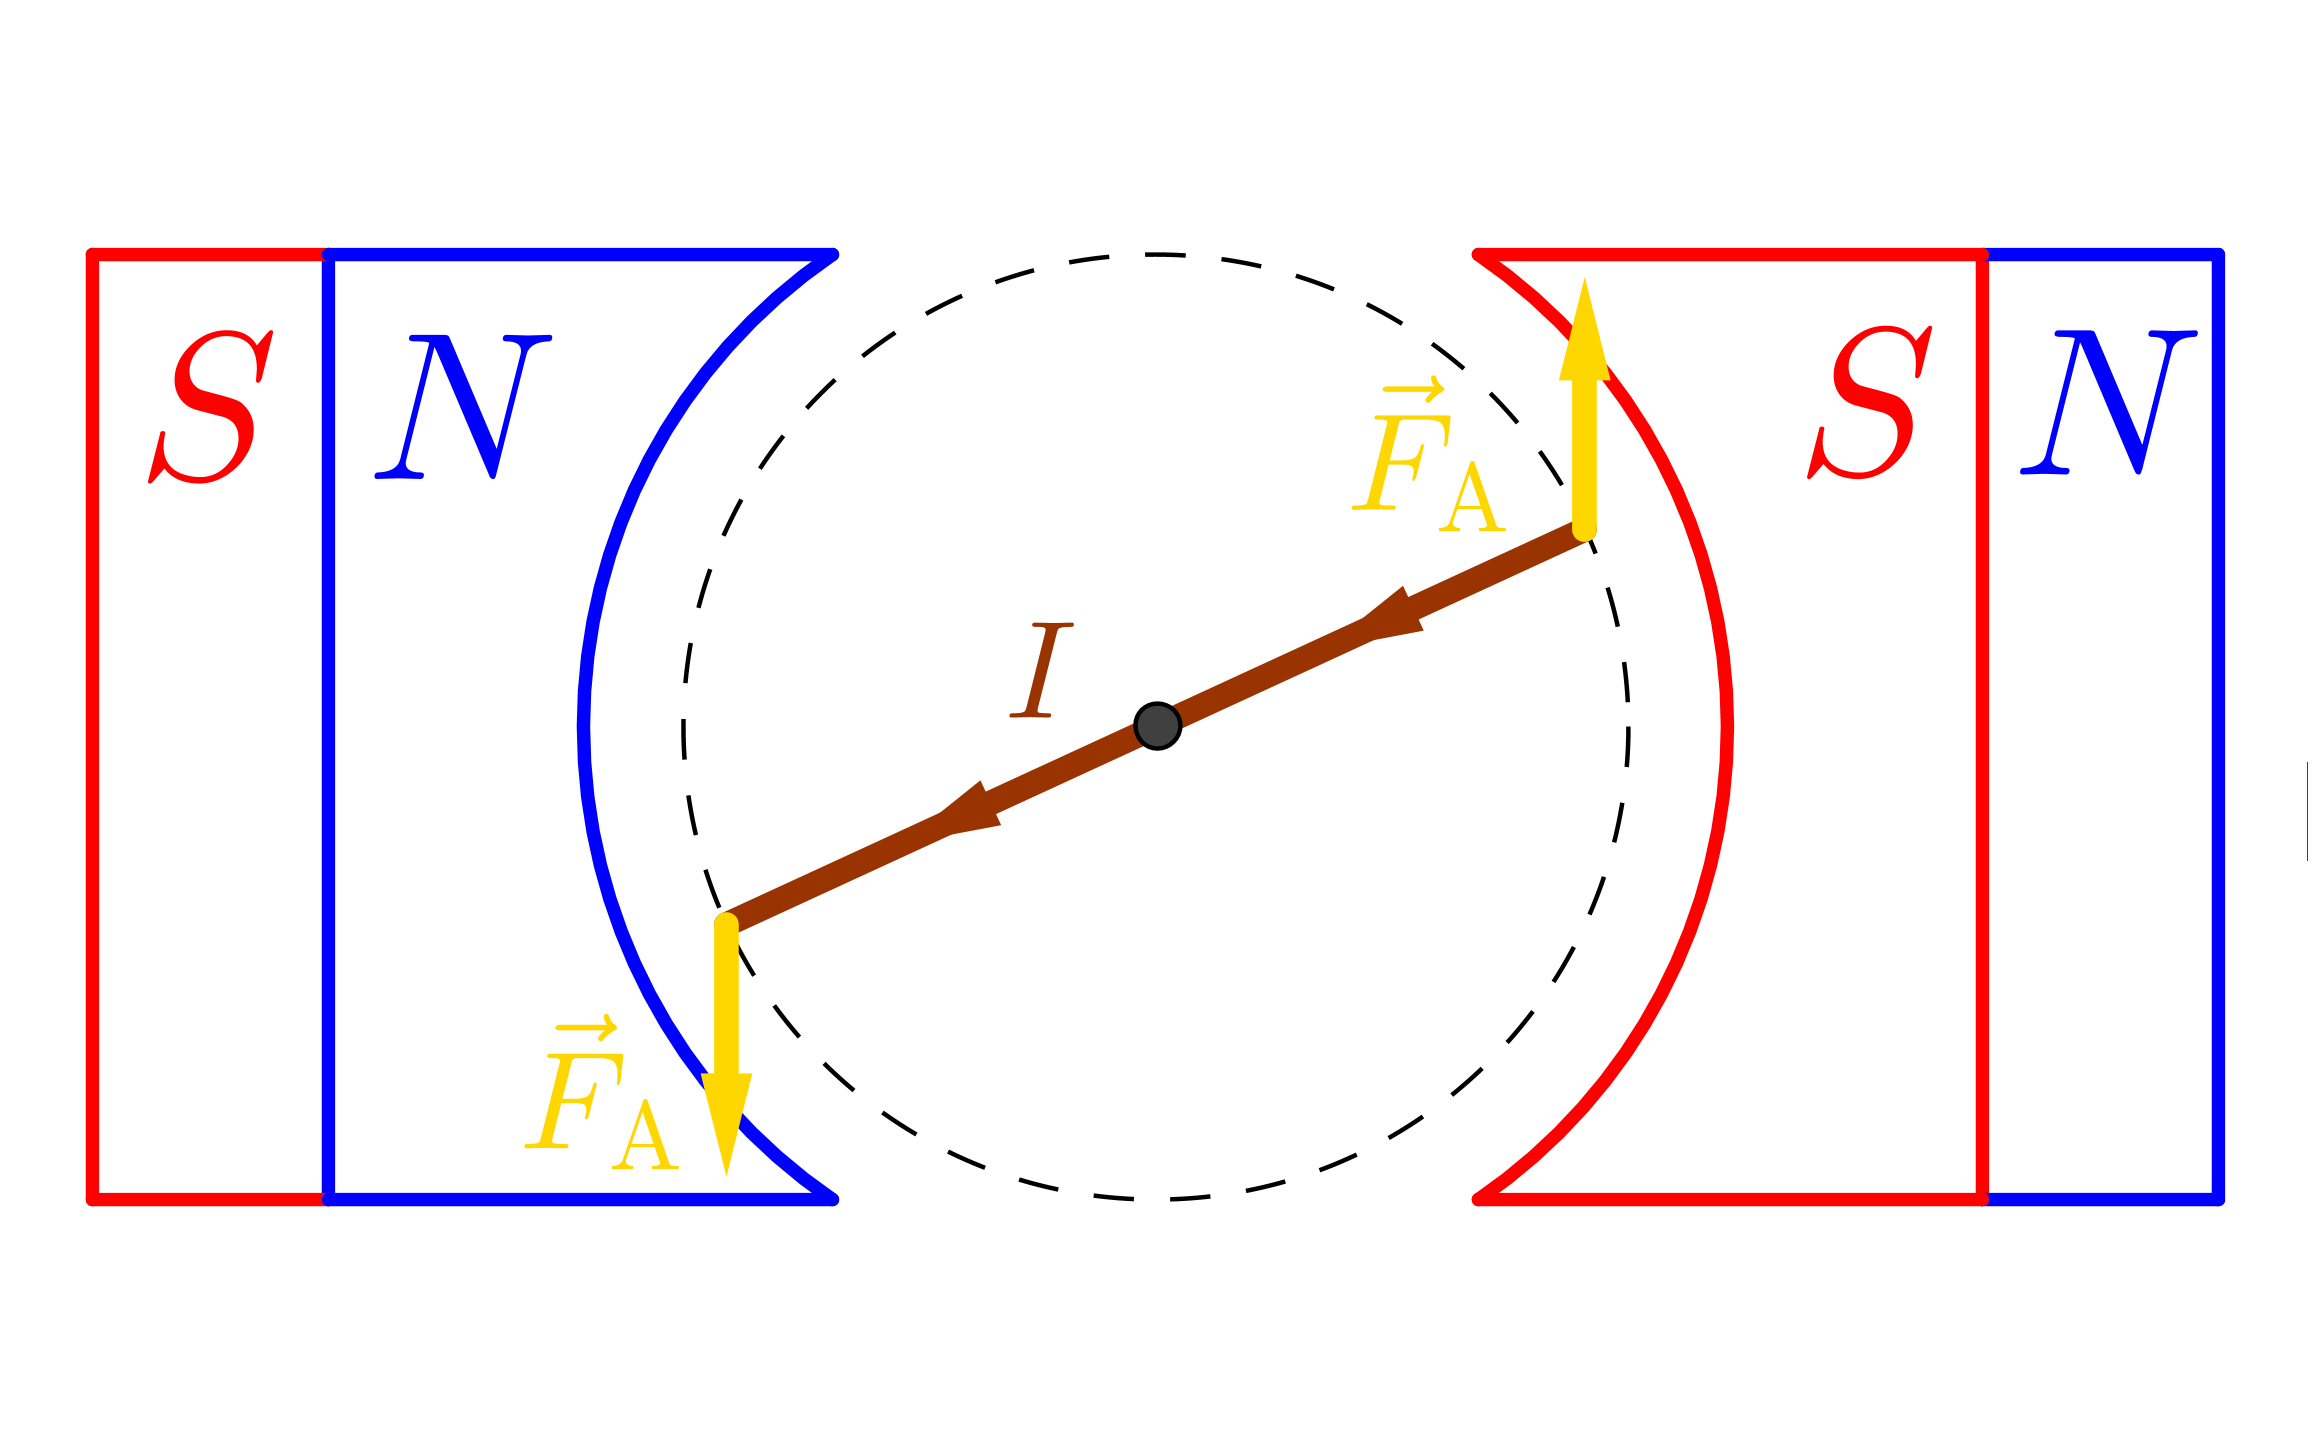
\includegraphics[height=5.5cm]{pics/phase_1.png}
			\caption{Начальное положение ротора.}
			\label{1_phase} 
		\end{minipage}
		\hfill 
		\begin{minipage}[h]{0.49\linewidth}
			\centering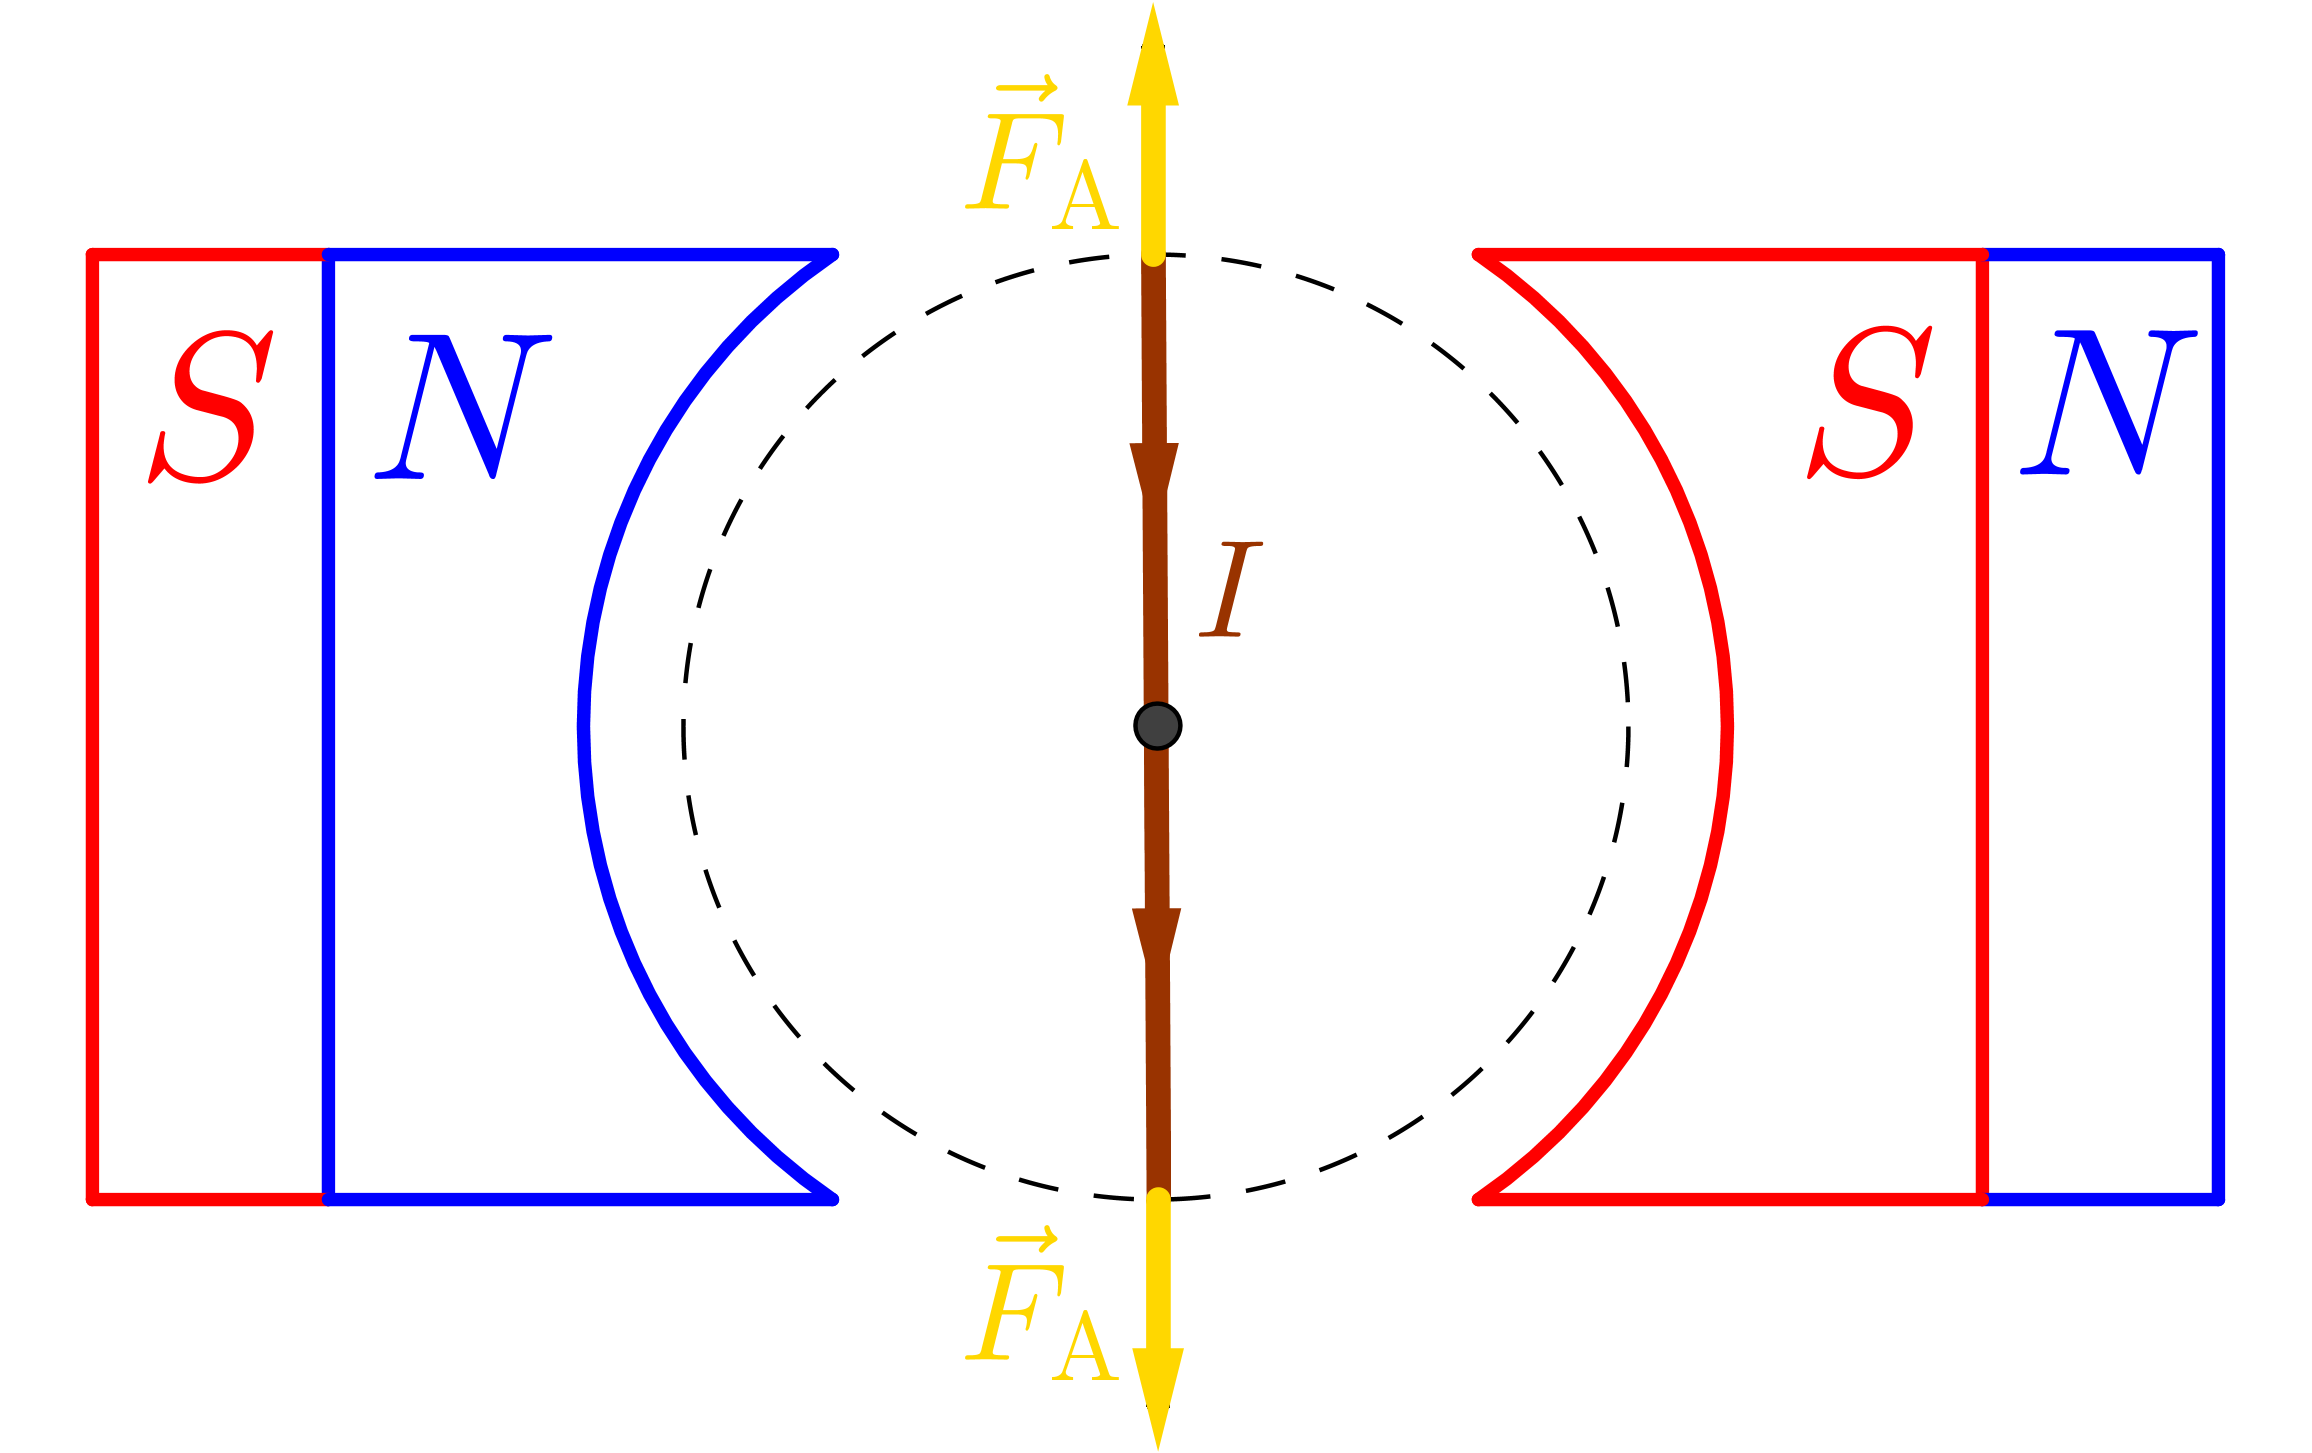
\includegraphics[height=5.5cm]{pics/phase_2.png}
			\caption{<<Переломный>> момент процесса.}
			\label{2_phase}
		\end{minipage}
	\end{center}
\end{figure}

Очевидно, что вплоть до достижения ротором двигателя положения, показанного на рис.~\ref{2_phase}, характер его движения меняться не будет: он, разгоняемый выше упомянутыми силами, так же будет продолжать свое движение против часовой стрелки. 
Что касается самой этой позиции, то, пусть в ней ротор не разгоняется силами Ампера, ее он все равно пройдет в силу инерции. 

Как следует из сказанного, далее ротор окажется в состоянии, изображенном на рис.~\ref{3_phase}. 
Но возникает вопрос: а как это может быть, ведь из рисунка ясно видно, что некогда разгонявшие ротор силы, отныне будут его тормозить, а возможно, даже и приведут его во вращение по часовой стрелки. 
Ответ на на него очевиден~--- для нормальной работы двигателя это, конечно, недопустимо.

\begin{figure}[h]
	\begin{center}
		\begin{minipage}[h]{0.49\linewidth}
			\centering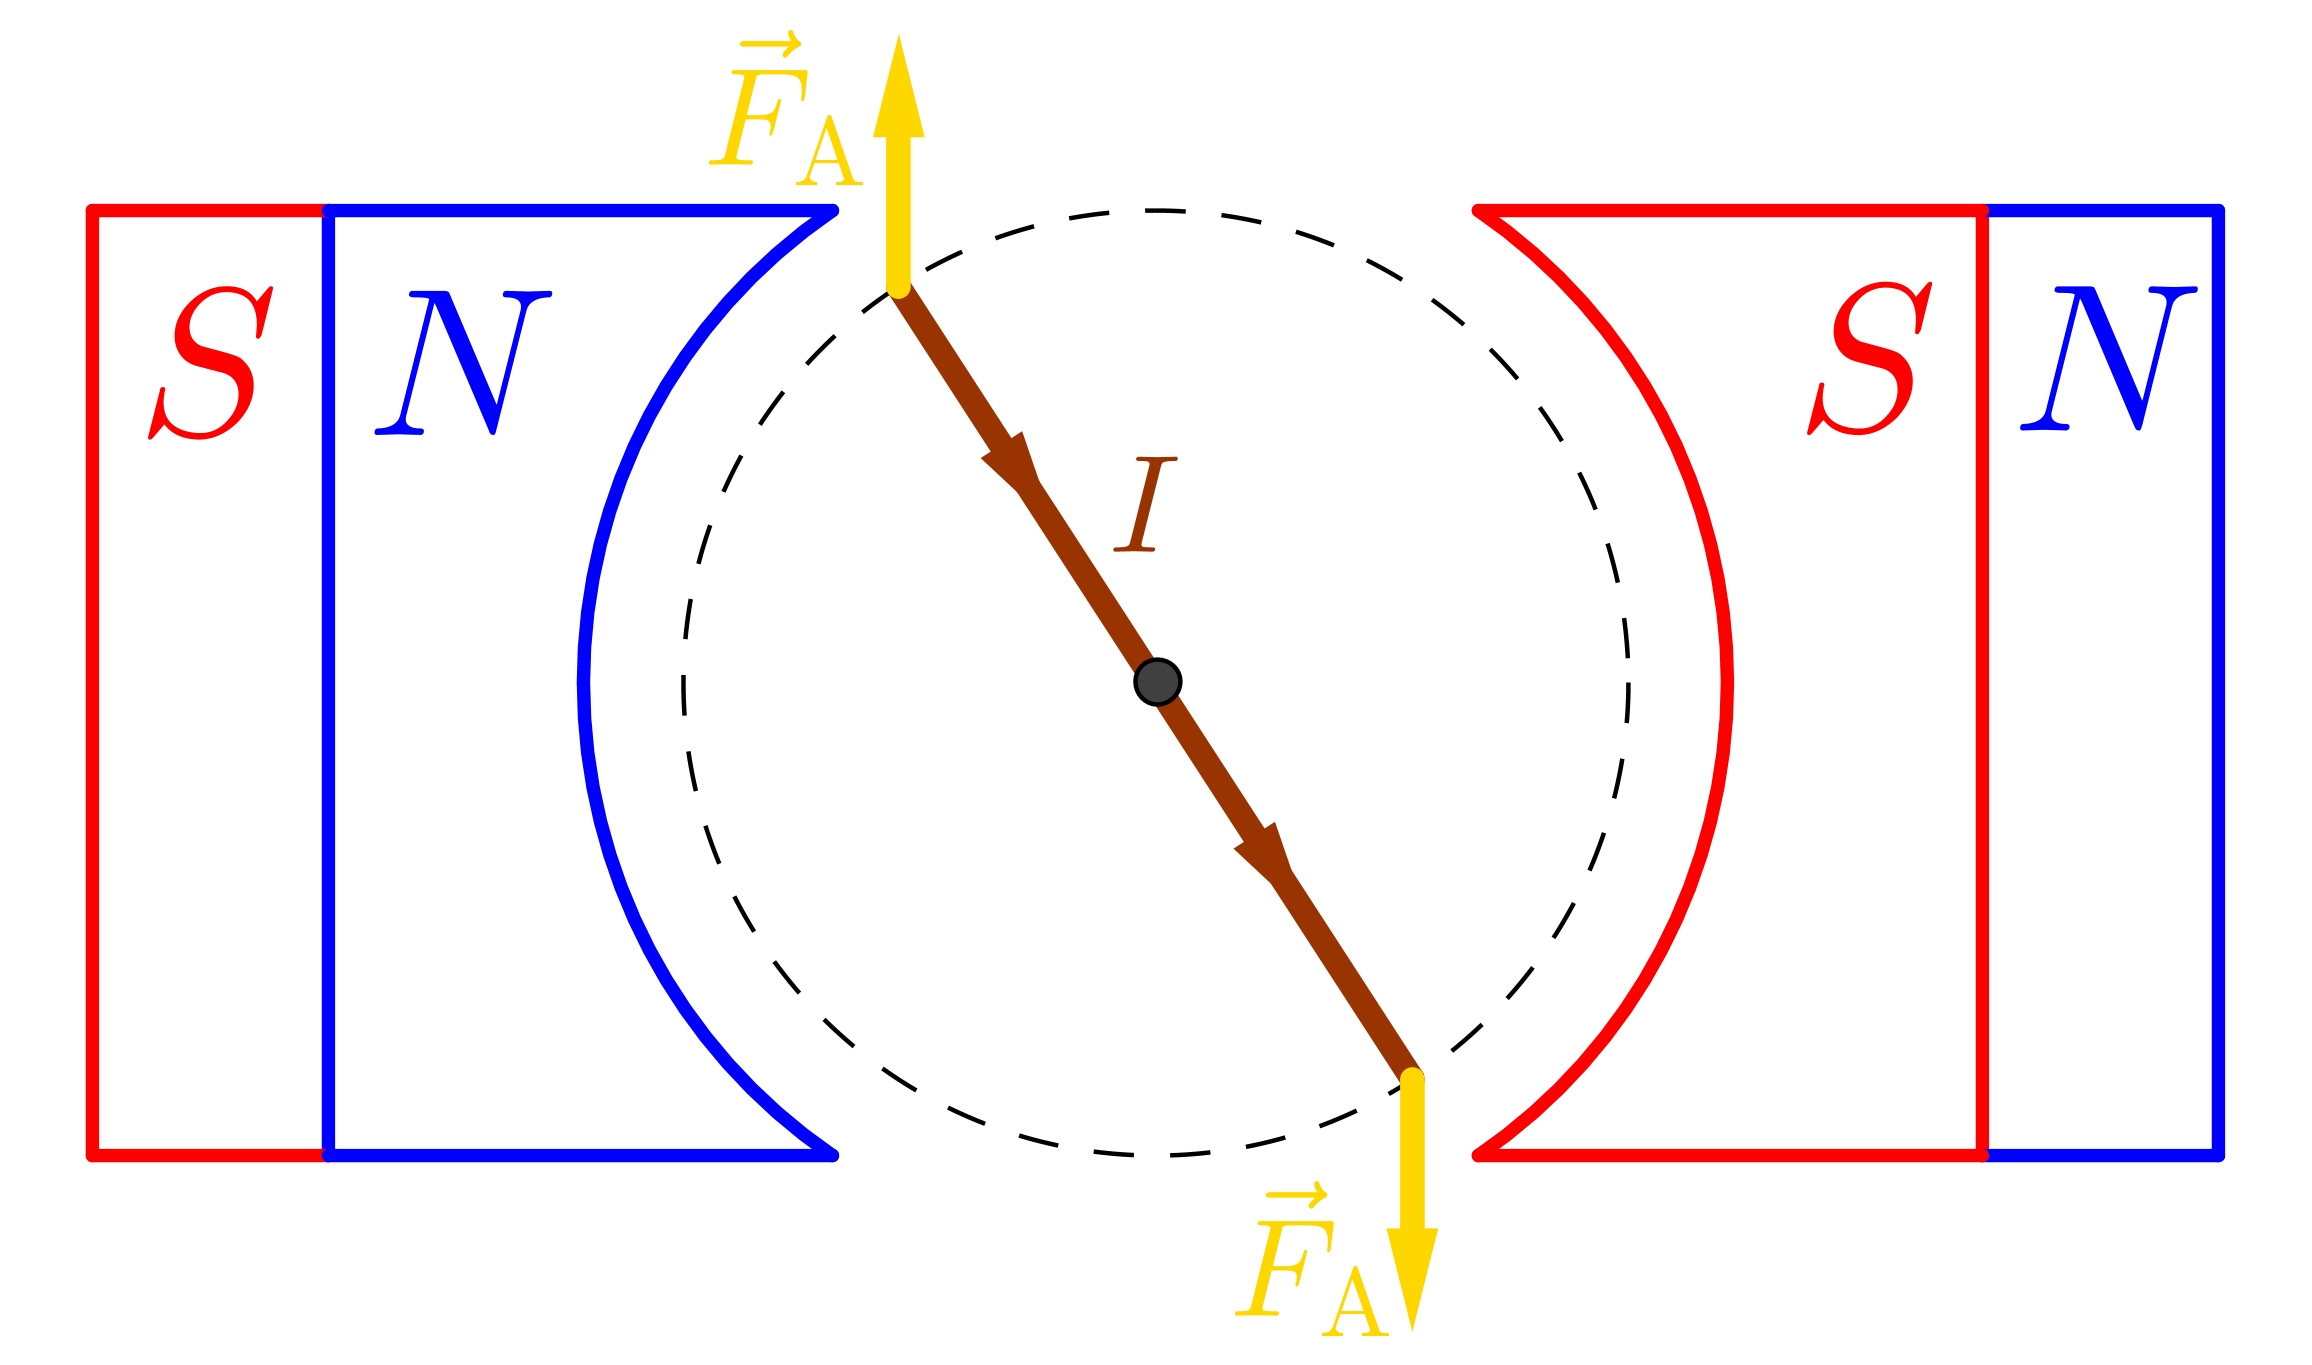
\includegraphics[height=5cm]{pics/phase_3.png}
			\caption{<<Парадокс>>.}
			\label{3_phase} 
		\end{minipage}
		\hfill 
		\begin{minipage}[h]{0.49\linewidth}
			\centering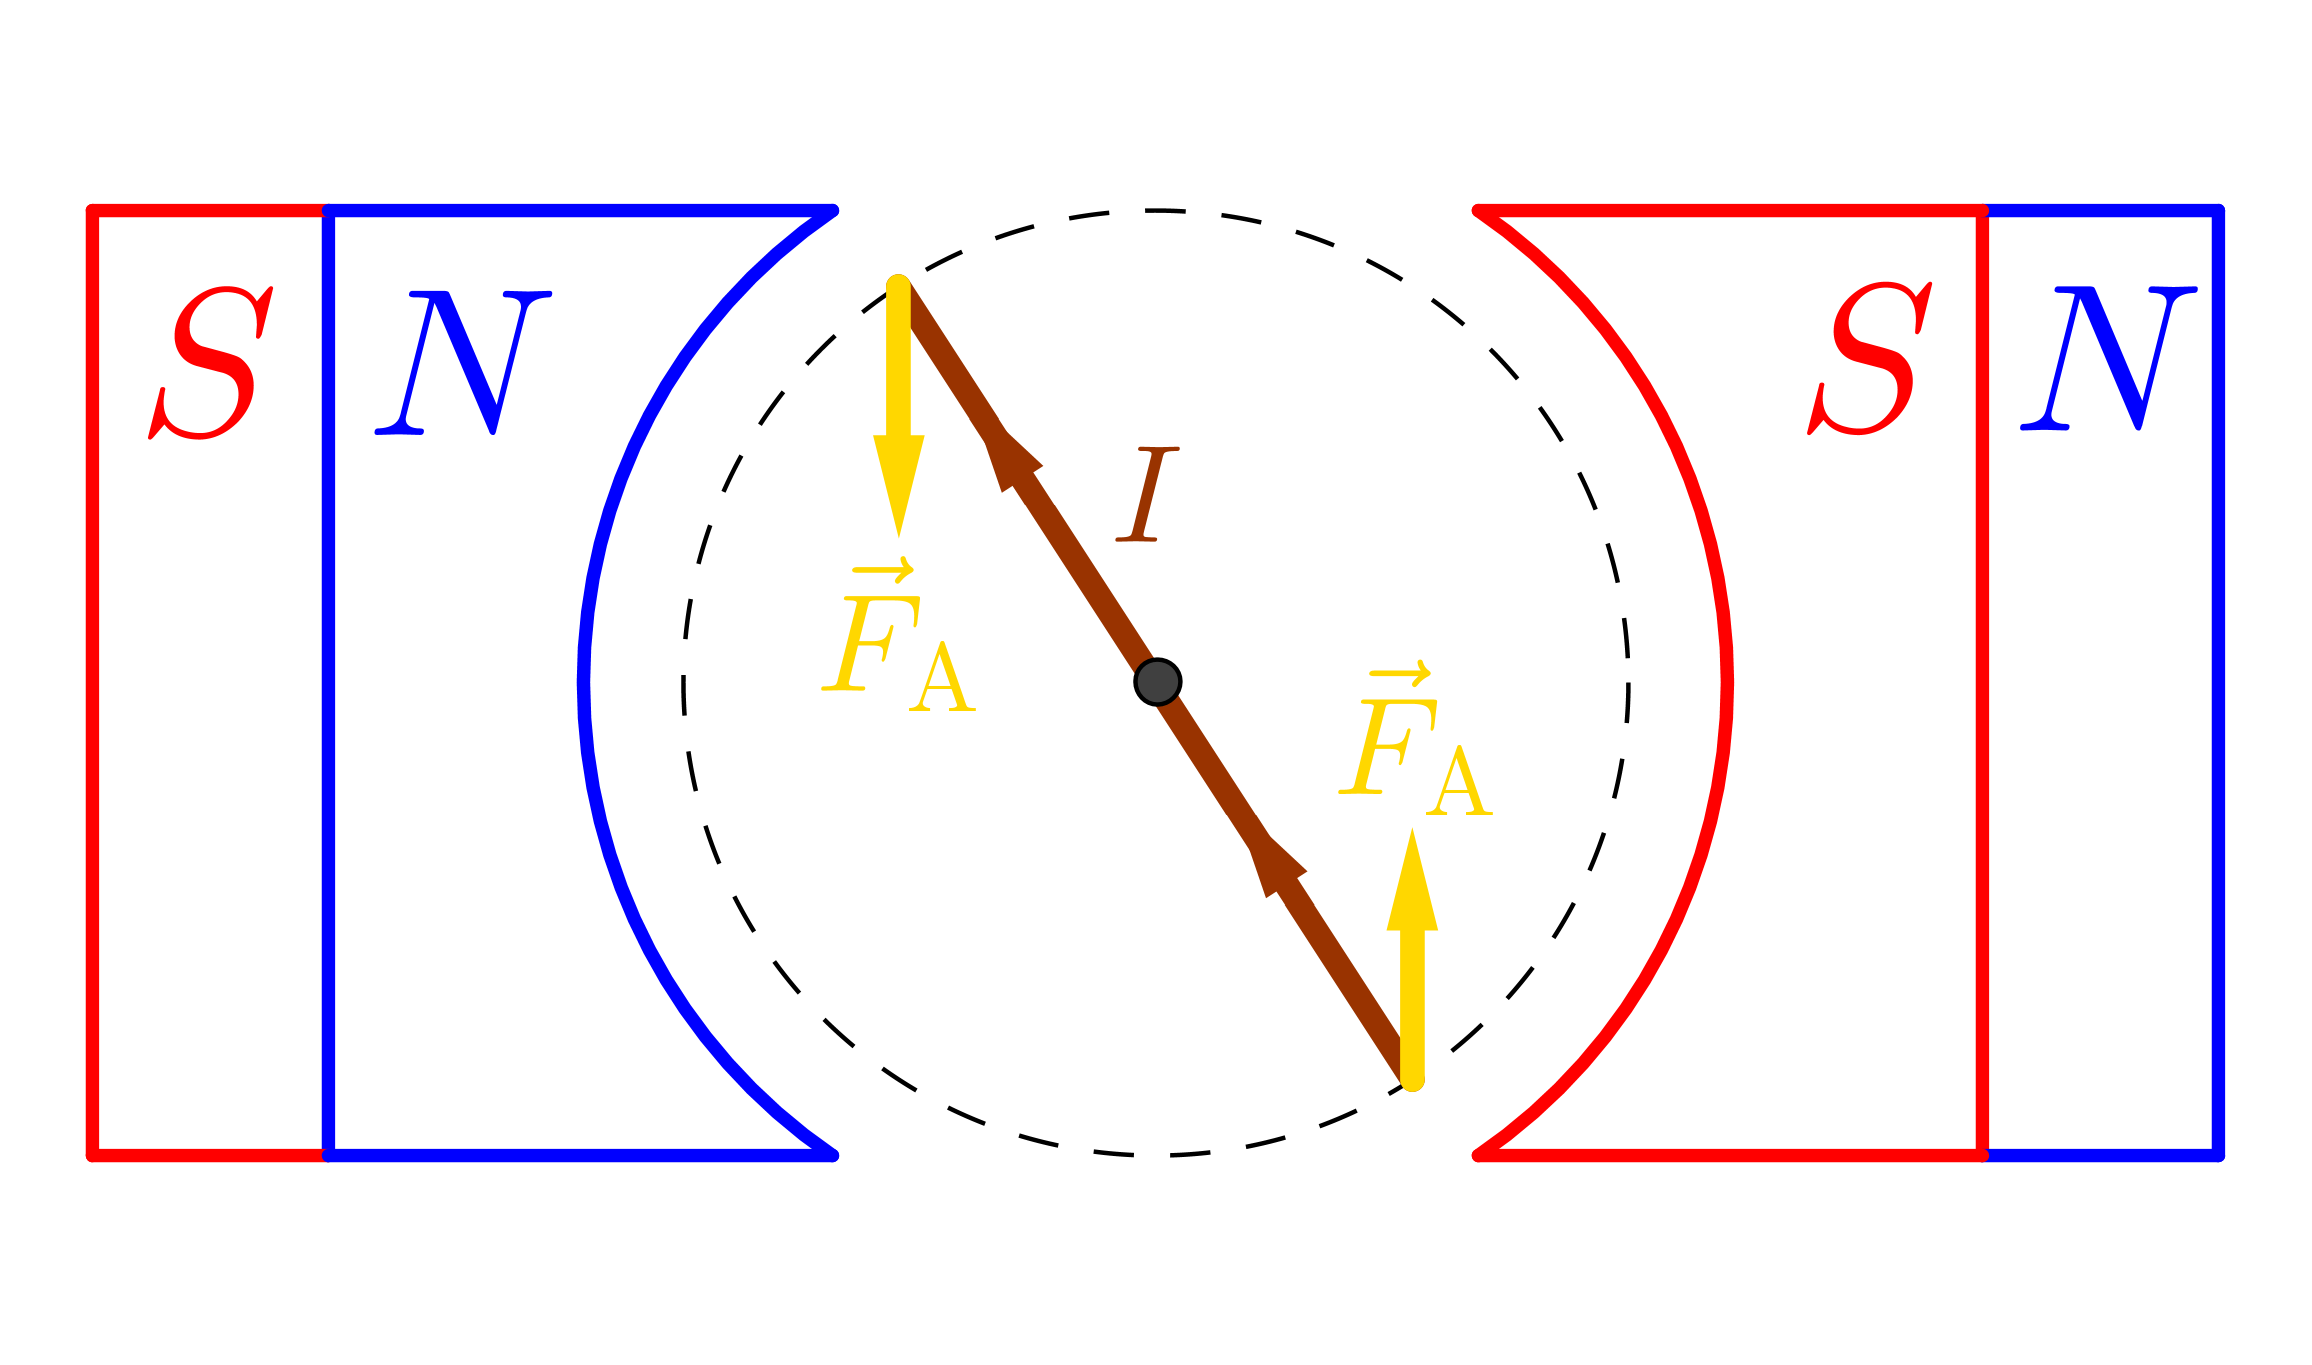
\includegraphics[height=5cm]{pics/phase_4.png}
			\caption{Действительная ситуация.}
			\label{4_phase}
		\end{minipage}
	\end{center}
\end{figure}

Пример решения этой проблемы, применяемого на практике, заключается в том, чтобы каждый раз после прохождения ротором положения, зафиксированного на рис.~\ref{2_phase}, менять направление тока в контуре на противоположное. 
В~этом случае все силы, действующие на стороны контура также поменяют направления на противоположные. 
Это, в свою очередь, означает, что ротор двигателя окажется в состоянии, изображенном на рис.~\ref{4_phase}, из которого видно, что при таком раскладе силы Амперы уже не будут создавать препятствий его дальнейшему движению.

Такое изменение направления тока можно легко реализовать, используя в качестве контактов контура два электрически изолированных друг от друга полуцилиндра (рис.~\ref{rotor_with_contacts}).
При этом необходимый эффект достигается, если напряжение на них подводить с помощью металлических щеток или пластин, как показано на рис.~\ref{contacts_in_work}\lefteqn{.}\footnote{Познавательно отметить, что изображенная на рис.~\ref{contacts_in_work} часть электродвигателя называется \textit{щеточно-коллекторным узлом}.} 
Принцип работы должен быть понятен из данных иллюстраций. 
Единственное, что здесь можно добавить~--- проводя качественную аналогию между положениями контактов и ротора, следует заметить, что положению контактов a) соответствует положение ротора, изображенное на рис.~\ref{1_phase}, положению б)~--- положение ротора с рис.~\ref{2_phase} и, наконец, положению в)~--- рис.~\ref{4_phase}.

\begin{figure}[h]
	\noindent\centering{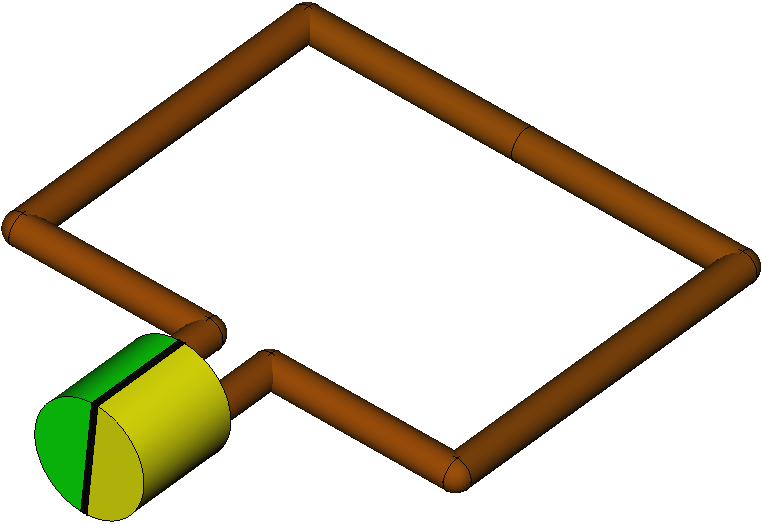
\includegraphics[scale=0.5]{pics/rotor_with_contacts_free.png}}
	\caption{Цилиндрические контакты на роторе.}
	\label{rotor_with_contacts}
\end{figure}

\begin{figure}[h]
	\begin{minipage}[h]{0.31\linewidth}
		\center{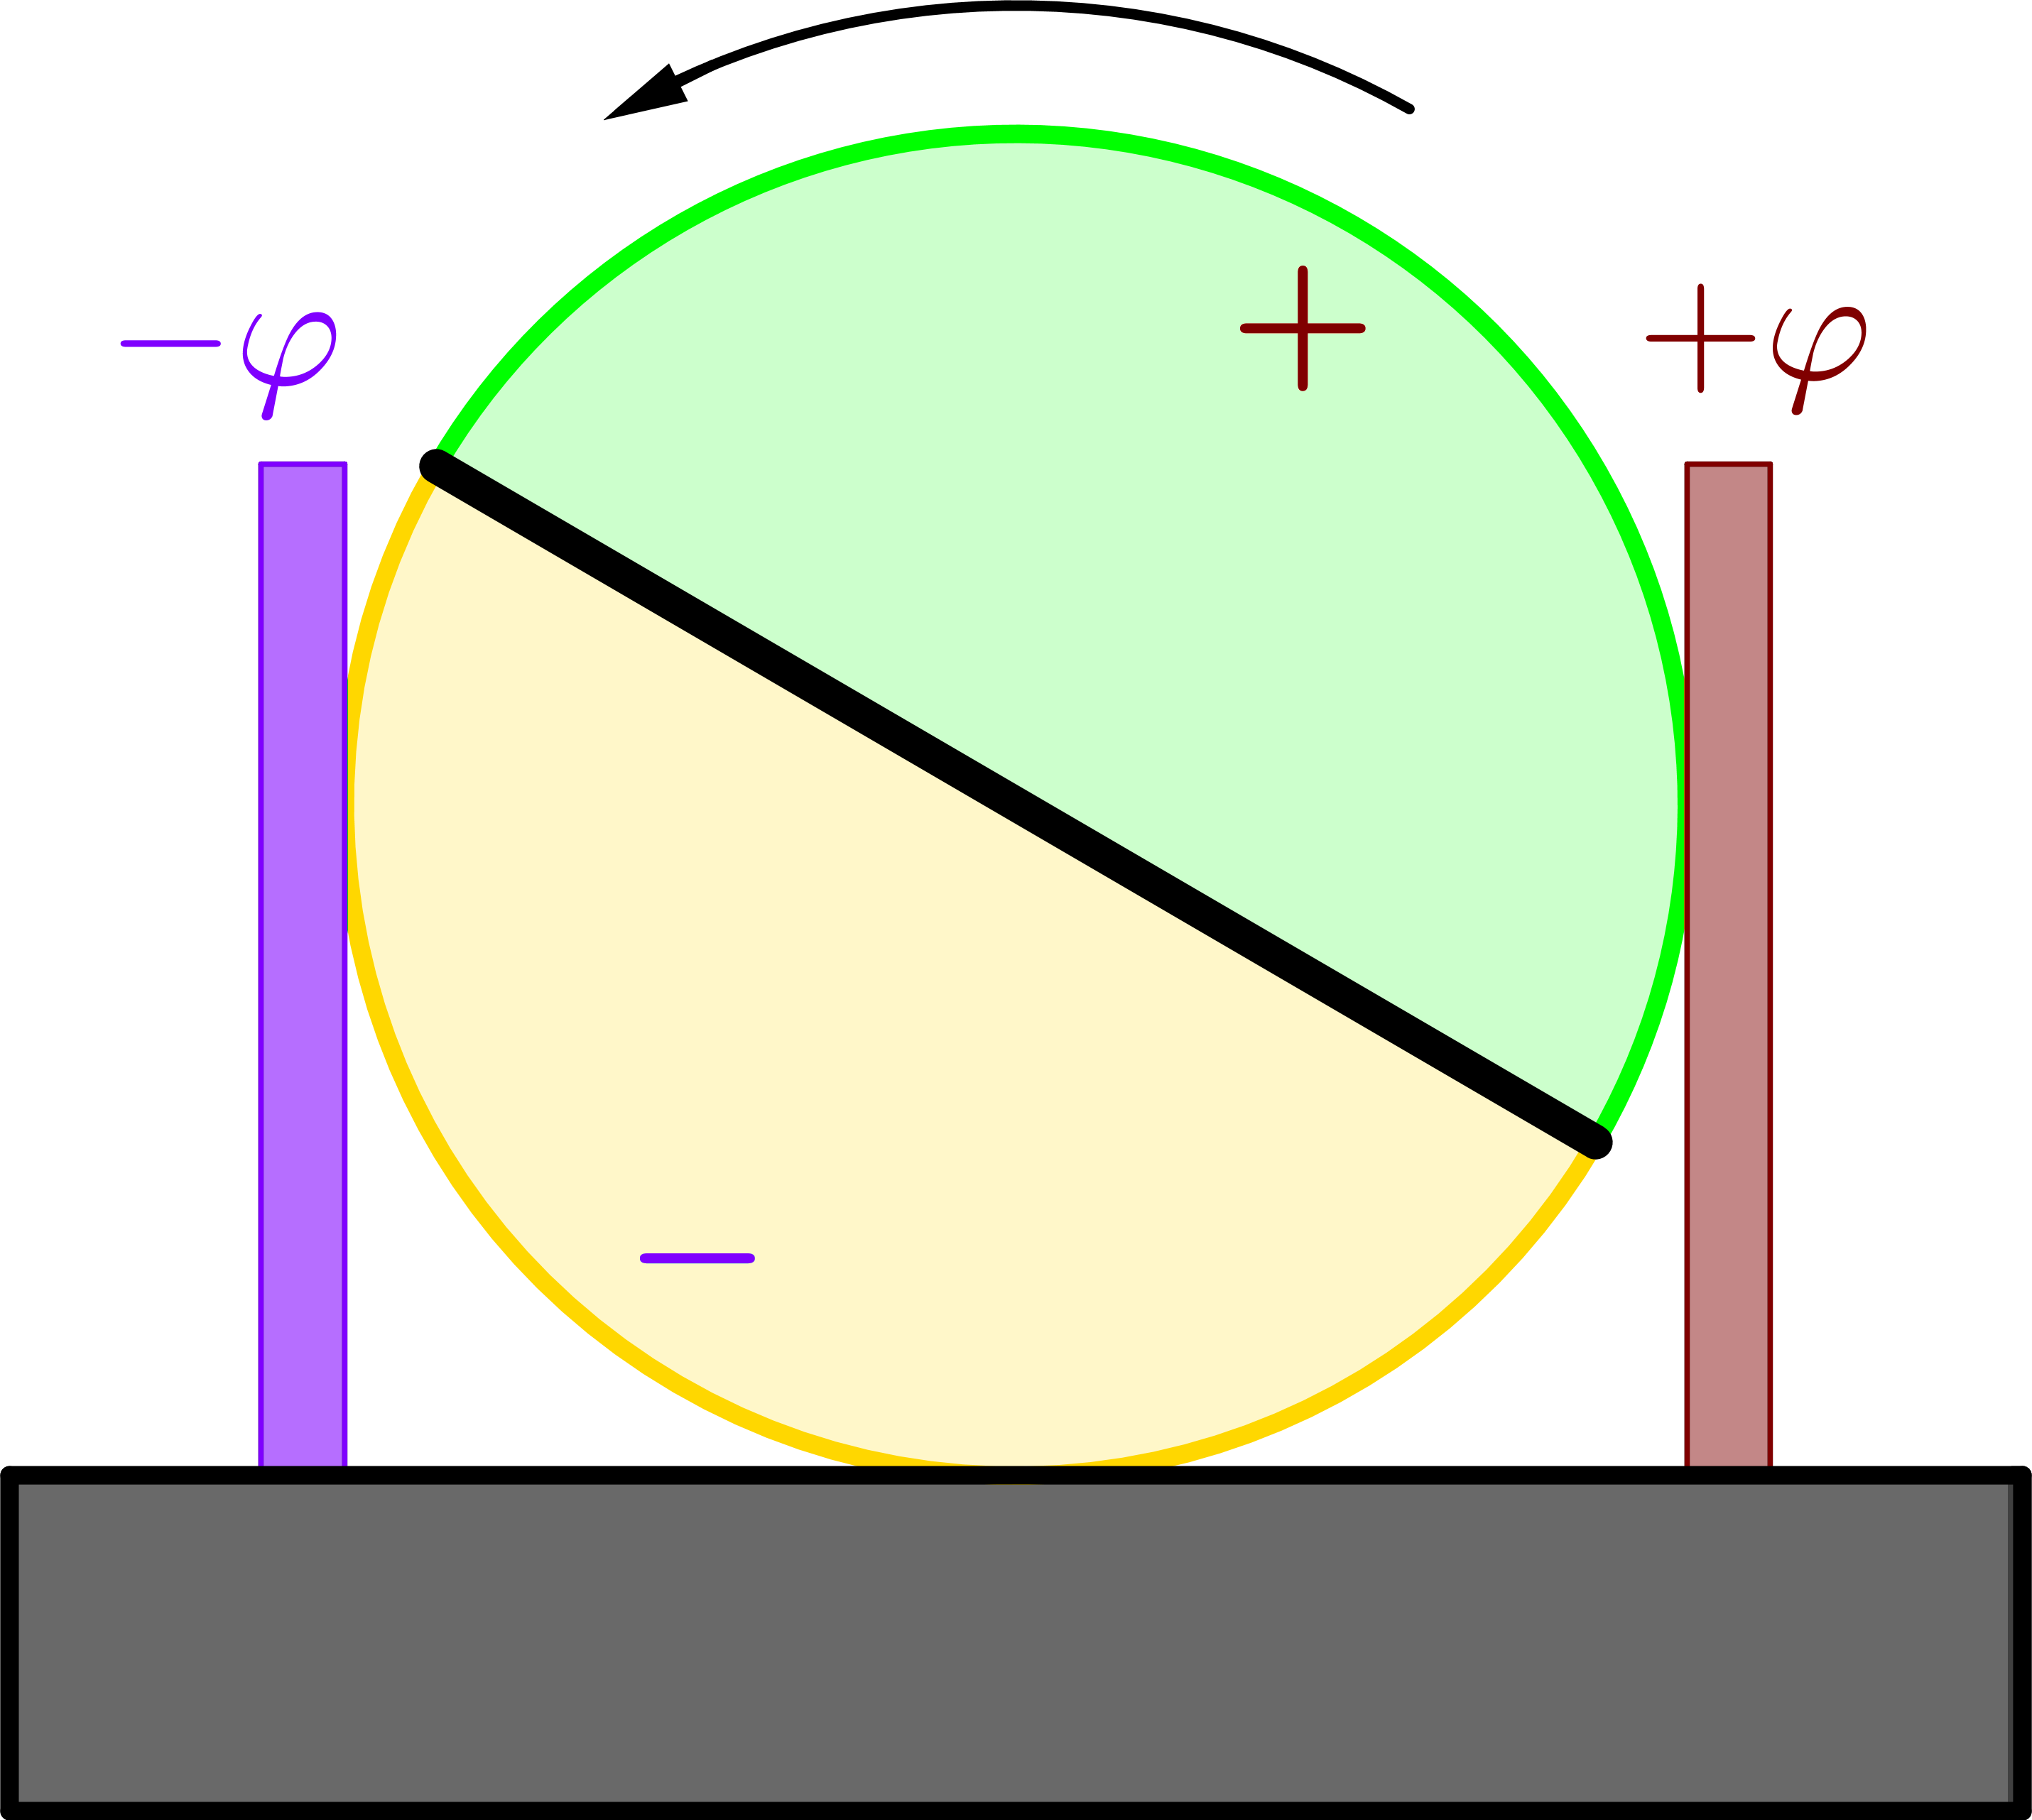
\includegraphics[width=\linewidth]{pics/contacts_phase_1.png}\\ а)}
	\end{minipage}
	\hfill
	\begin{minipage}[h]{0.31\linewidth}
		\center{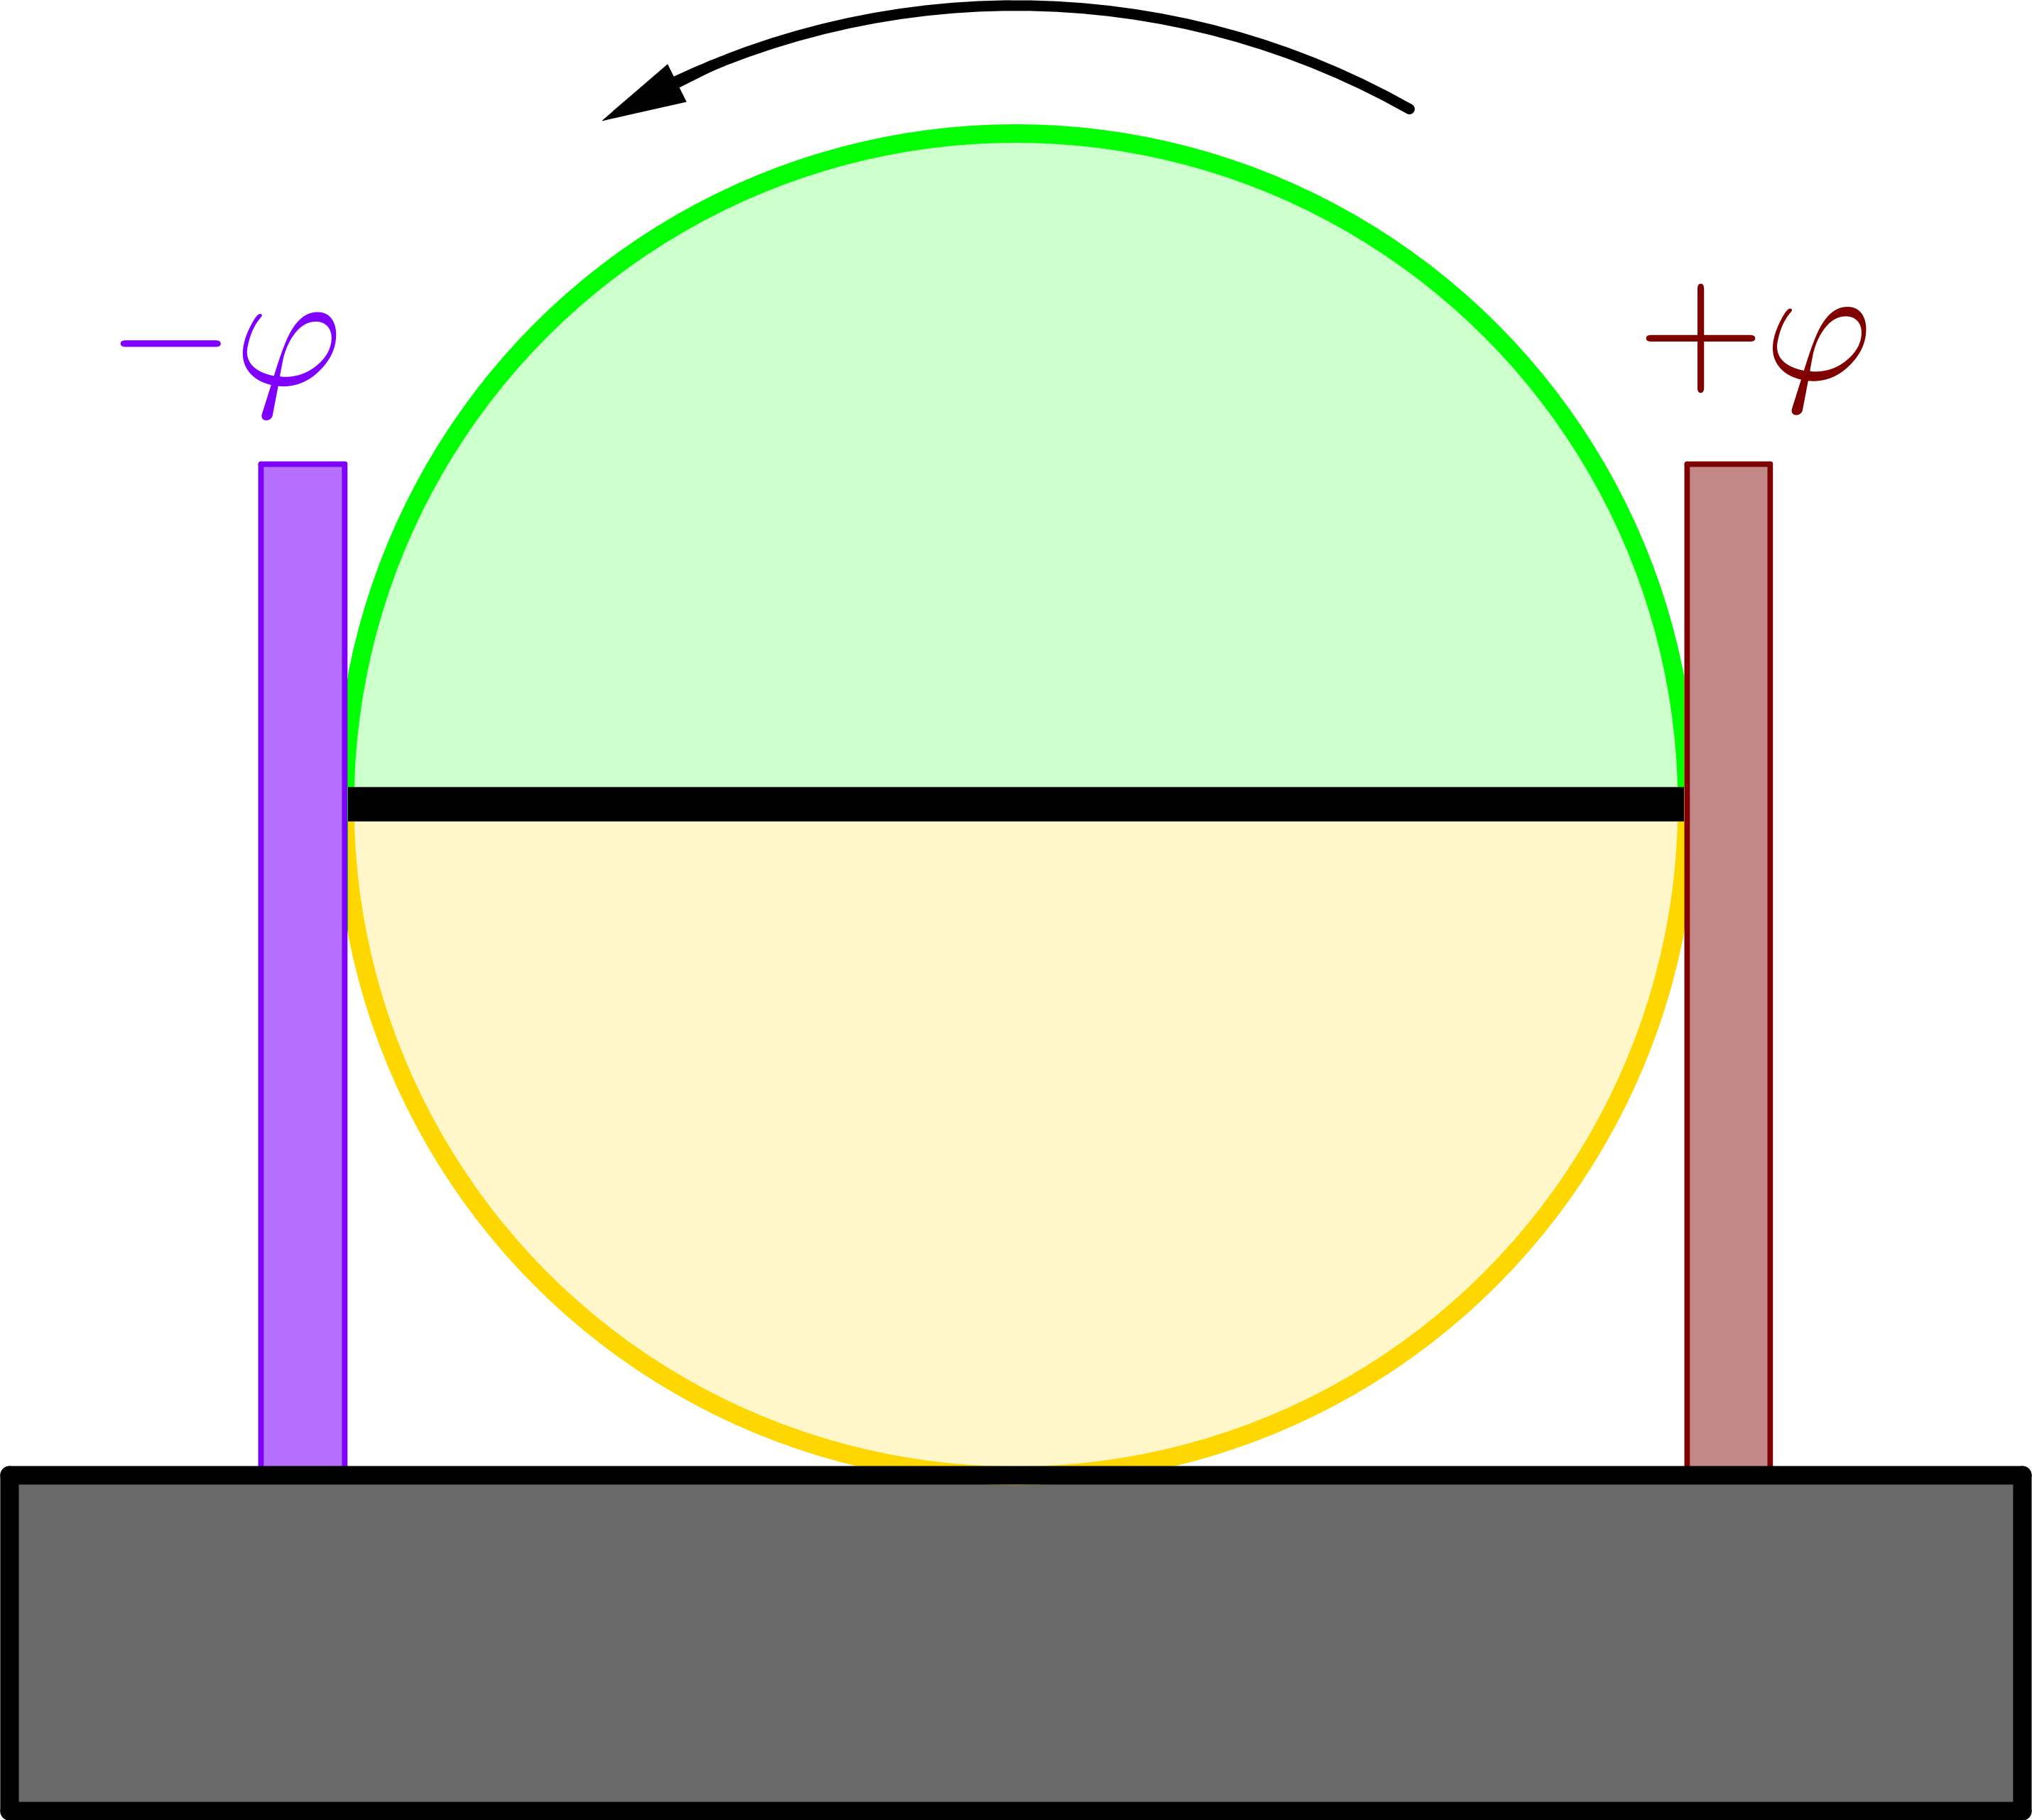
\includegraphics[width=\linewidth]{pics/contacts_phase_2.png}\\ б)}
	\end{minipage}
	\hfill
	\begin{minipage}[h]{0.31\linewidth}
		\center{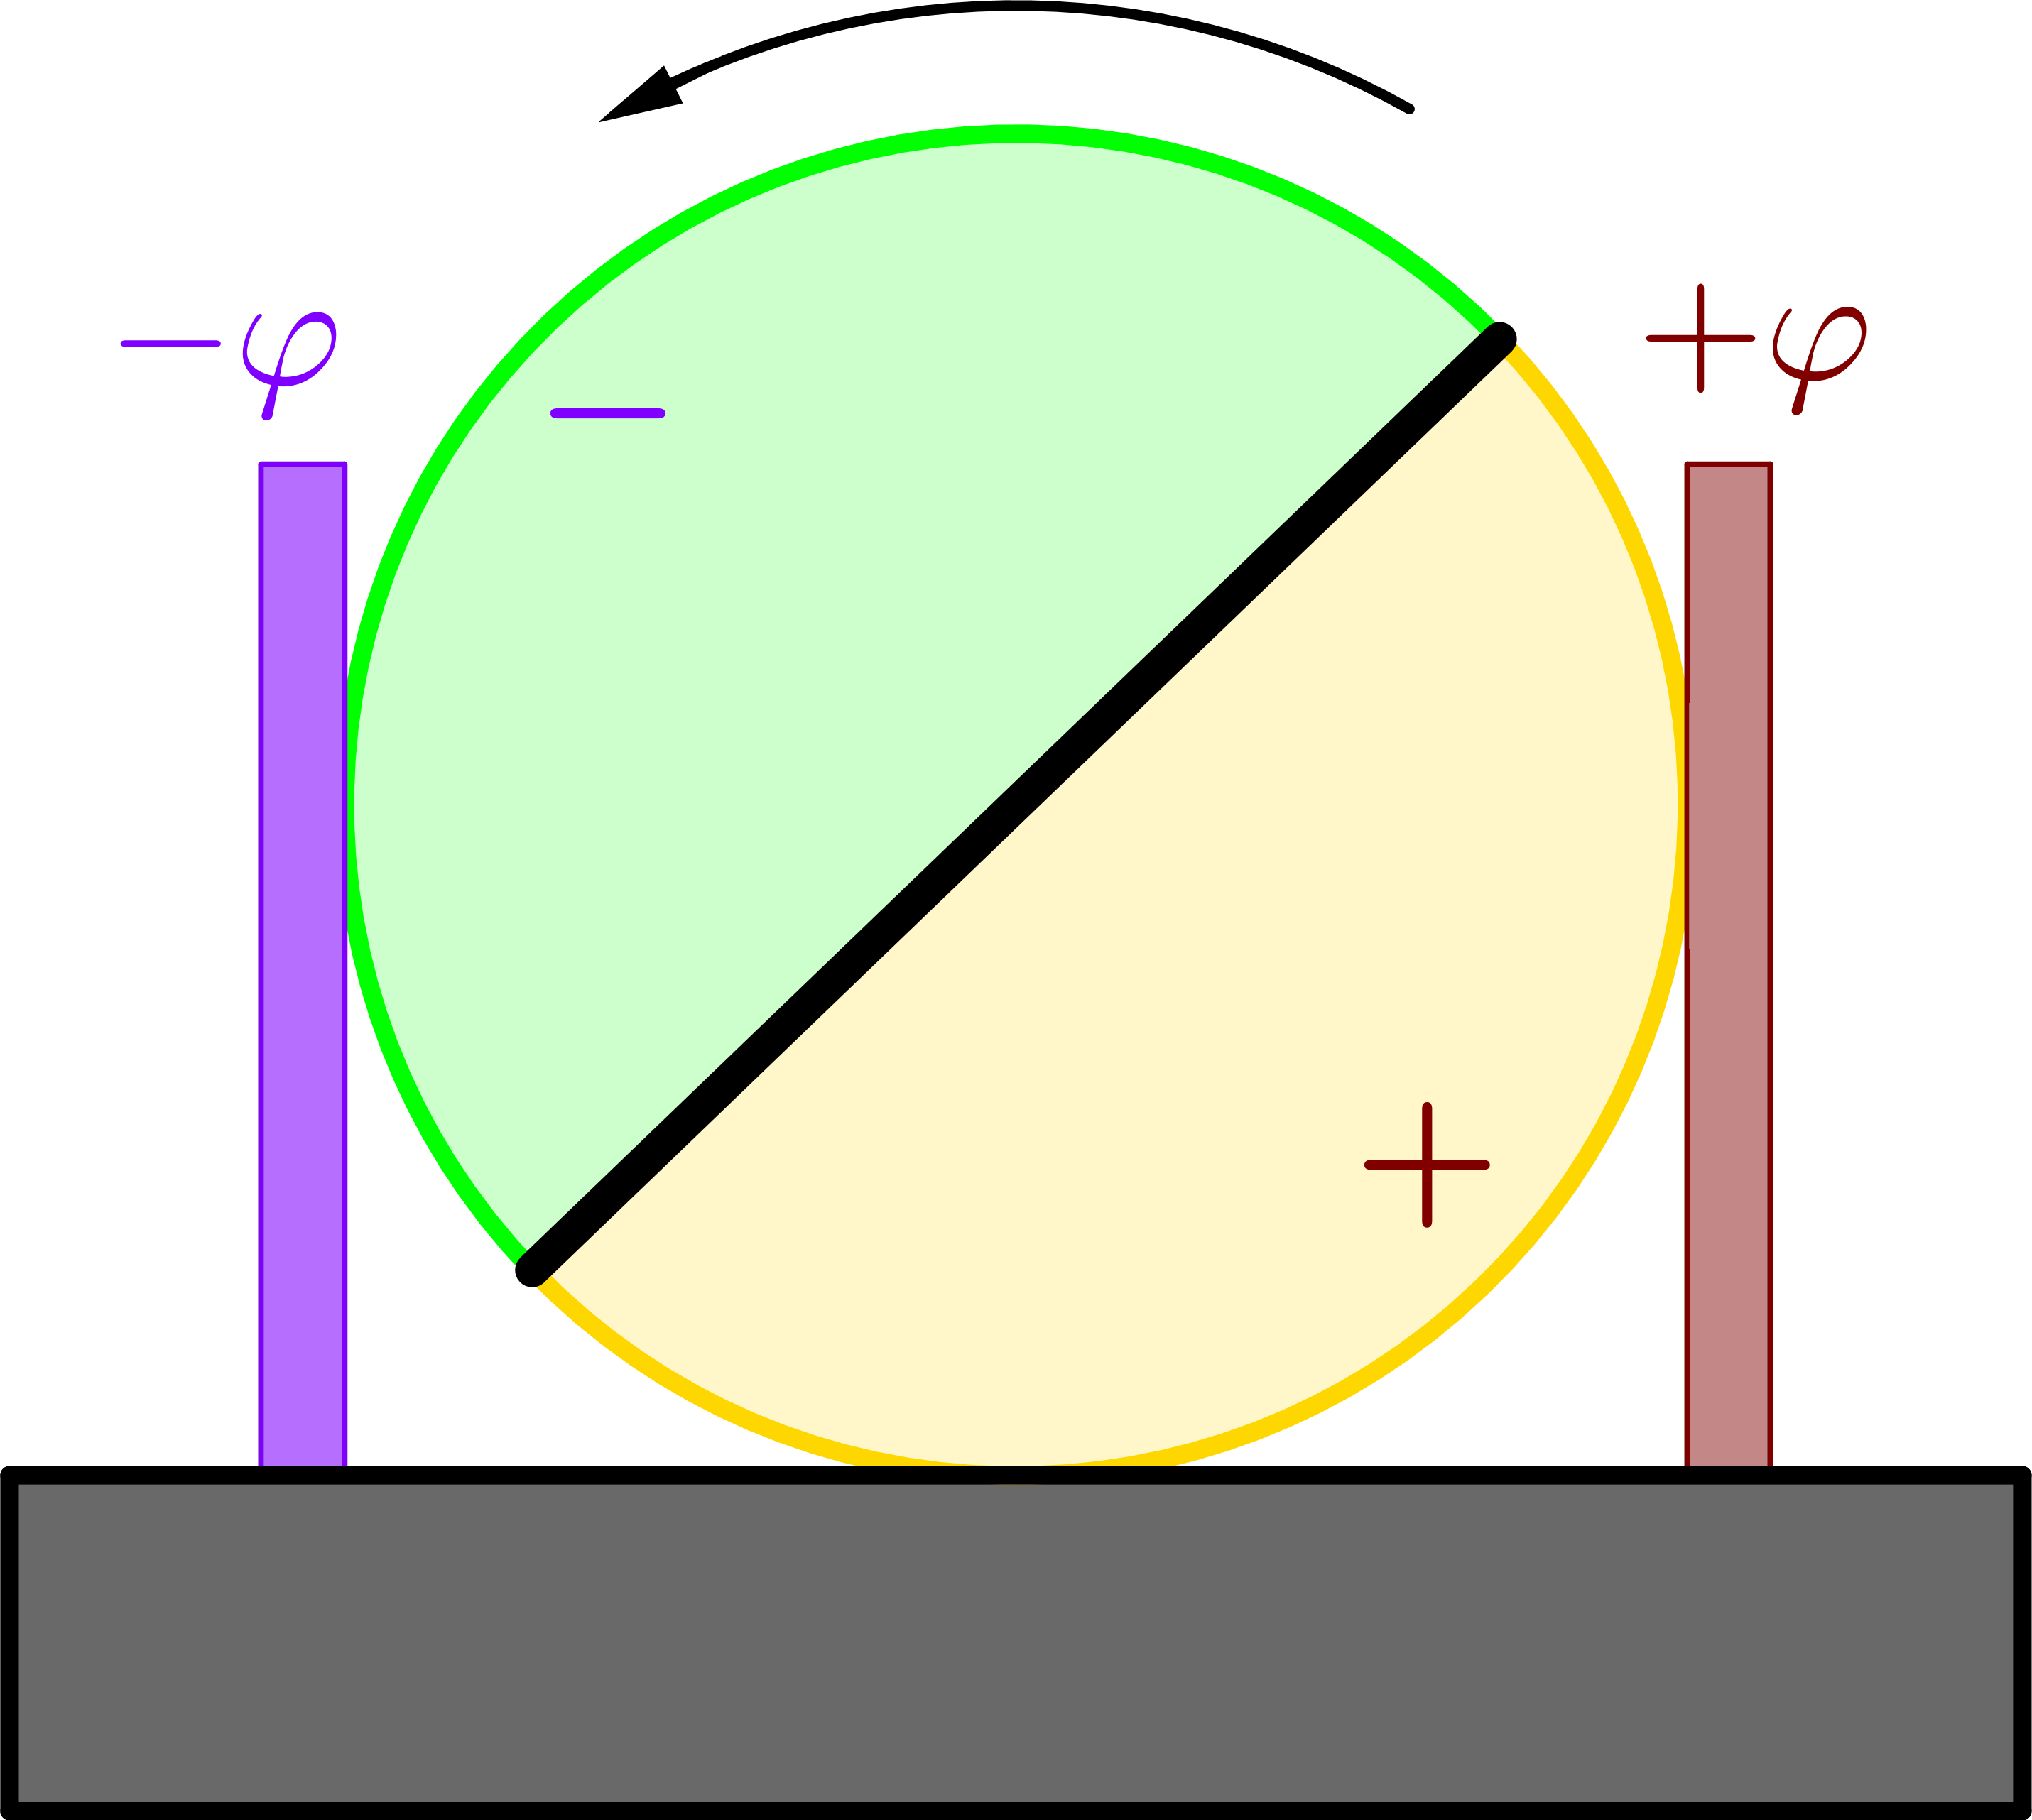
\includegraphics[width=\linewidth]{pics/contacts_phase_4.png}\\ в)}
	\end{minipage}
	\caption{Схема действия цилиндрических роторных контактов.}
	\label{contacts_in_work}
\end{figure}

Завершая рассмотрение строения двигателя, введем буквенные обозначения, описывающие его электродинамические параметры:
$R_\textit{р}$~--- сопротивление обмотки ротора;  $L_\textit{р}$~--- ее индуктивность.

%Возможно надо вставить эл. схему
\paragraph*{Математическая модель}$\phantom{-}$\\
\hspace*{\parindent}В~технических задачах, связанных с автоматическим управлением, все явления рассматриваются как некоторые {\itshape процессы}. 
Каждый из них прежде всего характеризуется\footnote{Следует отметить, что на самом деле в теории автоматического управления дается более сложная классификация характеристик процессов.}:
\begin{itemize}
\item {\itshape входными сигналами}~--- величинами, которые приводят к изменению текущего состояния системы и с помощью которых, следовательно, может осуществляться управление;
\item {\itshape выходными сигналами}~--- величинами, которые характеризуют состояние системы в данный момент времени и над которыми, соответственно, осуществляется управление;
\item функциональной зависимостью между ними~--- грубо говоря, информацией о том, как входные сигналы изменяют выходные.
\end{itemize} 

Рассматривая с учетом данной терминологии работу электродвигателя можно сказать следующее.

Роль входного сигнала выполняет подаваемое на двигатель напряжение ($U_{ctrl}$).
Действительно, ведь, например, для того, чтобы осуществить такое изменение состояния двигателя, как запустить его ротор на вращение, надо приложить к электродвигателю определенную разность потенциалов.
Входными сигналами также могут являться и некоторые из моментов сил, приложенных к ротору.
К~примеру, если повернуть вал ротора рукой, тем самым приложив к нему определенный момент, его состояние, очевидно, изменится.
Мы будем рассматривать только такие ситуации, в которых $M_{oth} = 0$, а значит двигатель испытывает действие всего одного управляющего воздействия~--- напряжения. 

В~качестве выходных сигналов можно рассматривать сразу несколько величин: во-первых, ими являются кинематические характеристики вращения ротора, то есть рассмотренные нами в прошлой работе функции $\varepsilon(t)$, $\omega(t)$ и $\theta(t)$, во-вторых, величины, описывающие протекающие в двигателе электродинамические процессы, например сила тока в обмотке якоря ($I$), в-третьих, любые другие величины, удовлетворяющие данному выше определению, например развиваемый двигателем момент силы, раскручивающий его ротор ($M_{el}$).
В~данной работе мы будем интересоваться значениями двух выходных сигналов: угловой скоростью вращения ротора $\omega(t)$ и силы тока в обмотке якоря $I(t)$.

Функциональная зависимость будет представлена уравнениями, составляющими математическую модель.

Теперь же учитывая все сказанное и возвращаясь к составлению математической модели двигателя постоянного тока, можно сделать вывод о том, что в ней должны рассматриваться упомянутые величины, играющие роль входных и выходных сигналов.
При этом несложно видеть, что полученная в прошлой лабораторной версия математической модели: 
\begin{equation}\label{from_lab_1}
	\dot{\omega}(t)=\frac{M_\varSigma(t)}J,
\end{equation}
не удовлетворяет данному условию (например в ней нет упоминания о функции $U_{ctrl}$).
Из этого следует, что она не является полной, а значит подлежит уточнению. 

С~указанной целью запишем для электрической цепи, содержащей наш двигатель, закон Ома:
\begin{equation}\label{Om's_law}
	U_{ctrl} - \mathcal E_i - L_\textit{р}\frac{dI}{dt} = I\left(R_\textit{р} + R_\textit{п}\right),
\end{equation}
где $U_{ctrl}$~--- ЭДС источника тока; $\mathcal E_i$~--- ЭДС индукции, возникающая в обмотке якоря из-за его вращения; $L_\textit{р}\dot{I}$~--- ЭДС самоиндукции, возникающая вследствие изменения силы тока в обмотке (в первой работе этим слагаемым мы пренебрегли); $R_\textit{п}$~--- суммарное сопротивление всех остальных проводников цепи кроме обмотки якоря, то есть $R_\textit{р} + R_\textit{п} = R$, где $R$~--- полное сопротивление цепи.
Все величины, входящие в это выражение, кроме $R_\textit{р}$, $R_\textit{п}$ и $L_\textit{р}$ следует рассматривать, как функции от времени. 
Выполняется оно всегда, несмотря на то, что сила тока в обмотке периодически меняет направление.

Чтобы убедиться в истинности правой части уравнения~\eqref{Om's_law}, в частности именно в такой постановке знаков, рассмотрим поворот якоря из состояния, изображенного на рис.~\ref{1_phase} в положение, зафиксированное на рис.~\ref{2_phase}.

При указанном повороте, как видно, например, из рис.~\ref{inductions}, поток магнитного поля $\vec B$, создаваемого статором, через контур будет возрастать.
Его изменение (возрастание), согласно \textit{явлению электромагнитной индукции}, спровоцирует появление в контуре индуцированного тока.
Направление последнего, согласно \textit{правилу Ленца}, будет таким, чтобы создаваемое им магнитное поле $\vec B_{\mathcal{E}_i}$ противодействовало имеющемуся изменению магнитного потока, обусловленного внешним магнитным полем $\vec B$, то есть в нашем случае уменьшало его (поток).
Этому будет соответствовать направление магнитного поля $\vec B_{\mathcal{E}_i}$, показанное на рис.~\ref{inductions} темно-зеленым цветом.
Согласно \textit{правилу буравчика}, такое магнитное поле создается током, противоположным по направлению контурному току.
Последнее же и означает, что перед $\mathcal E_i$ в выражении~\eqref{Om's_law} следует поставить минус.

\begin{figure}[h]
	\noindent\centering{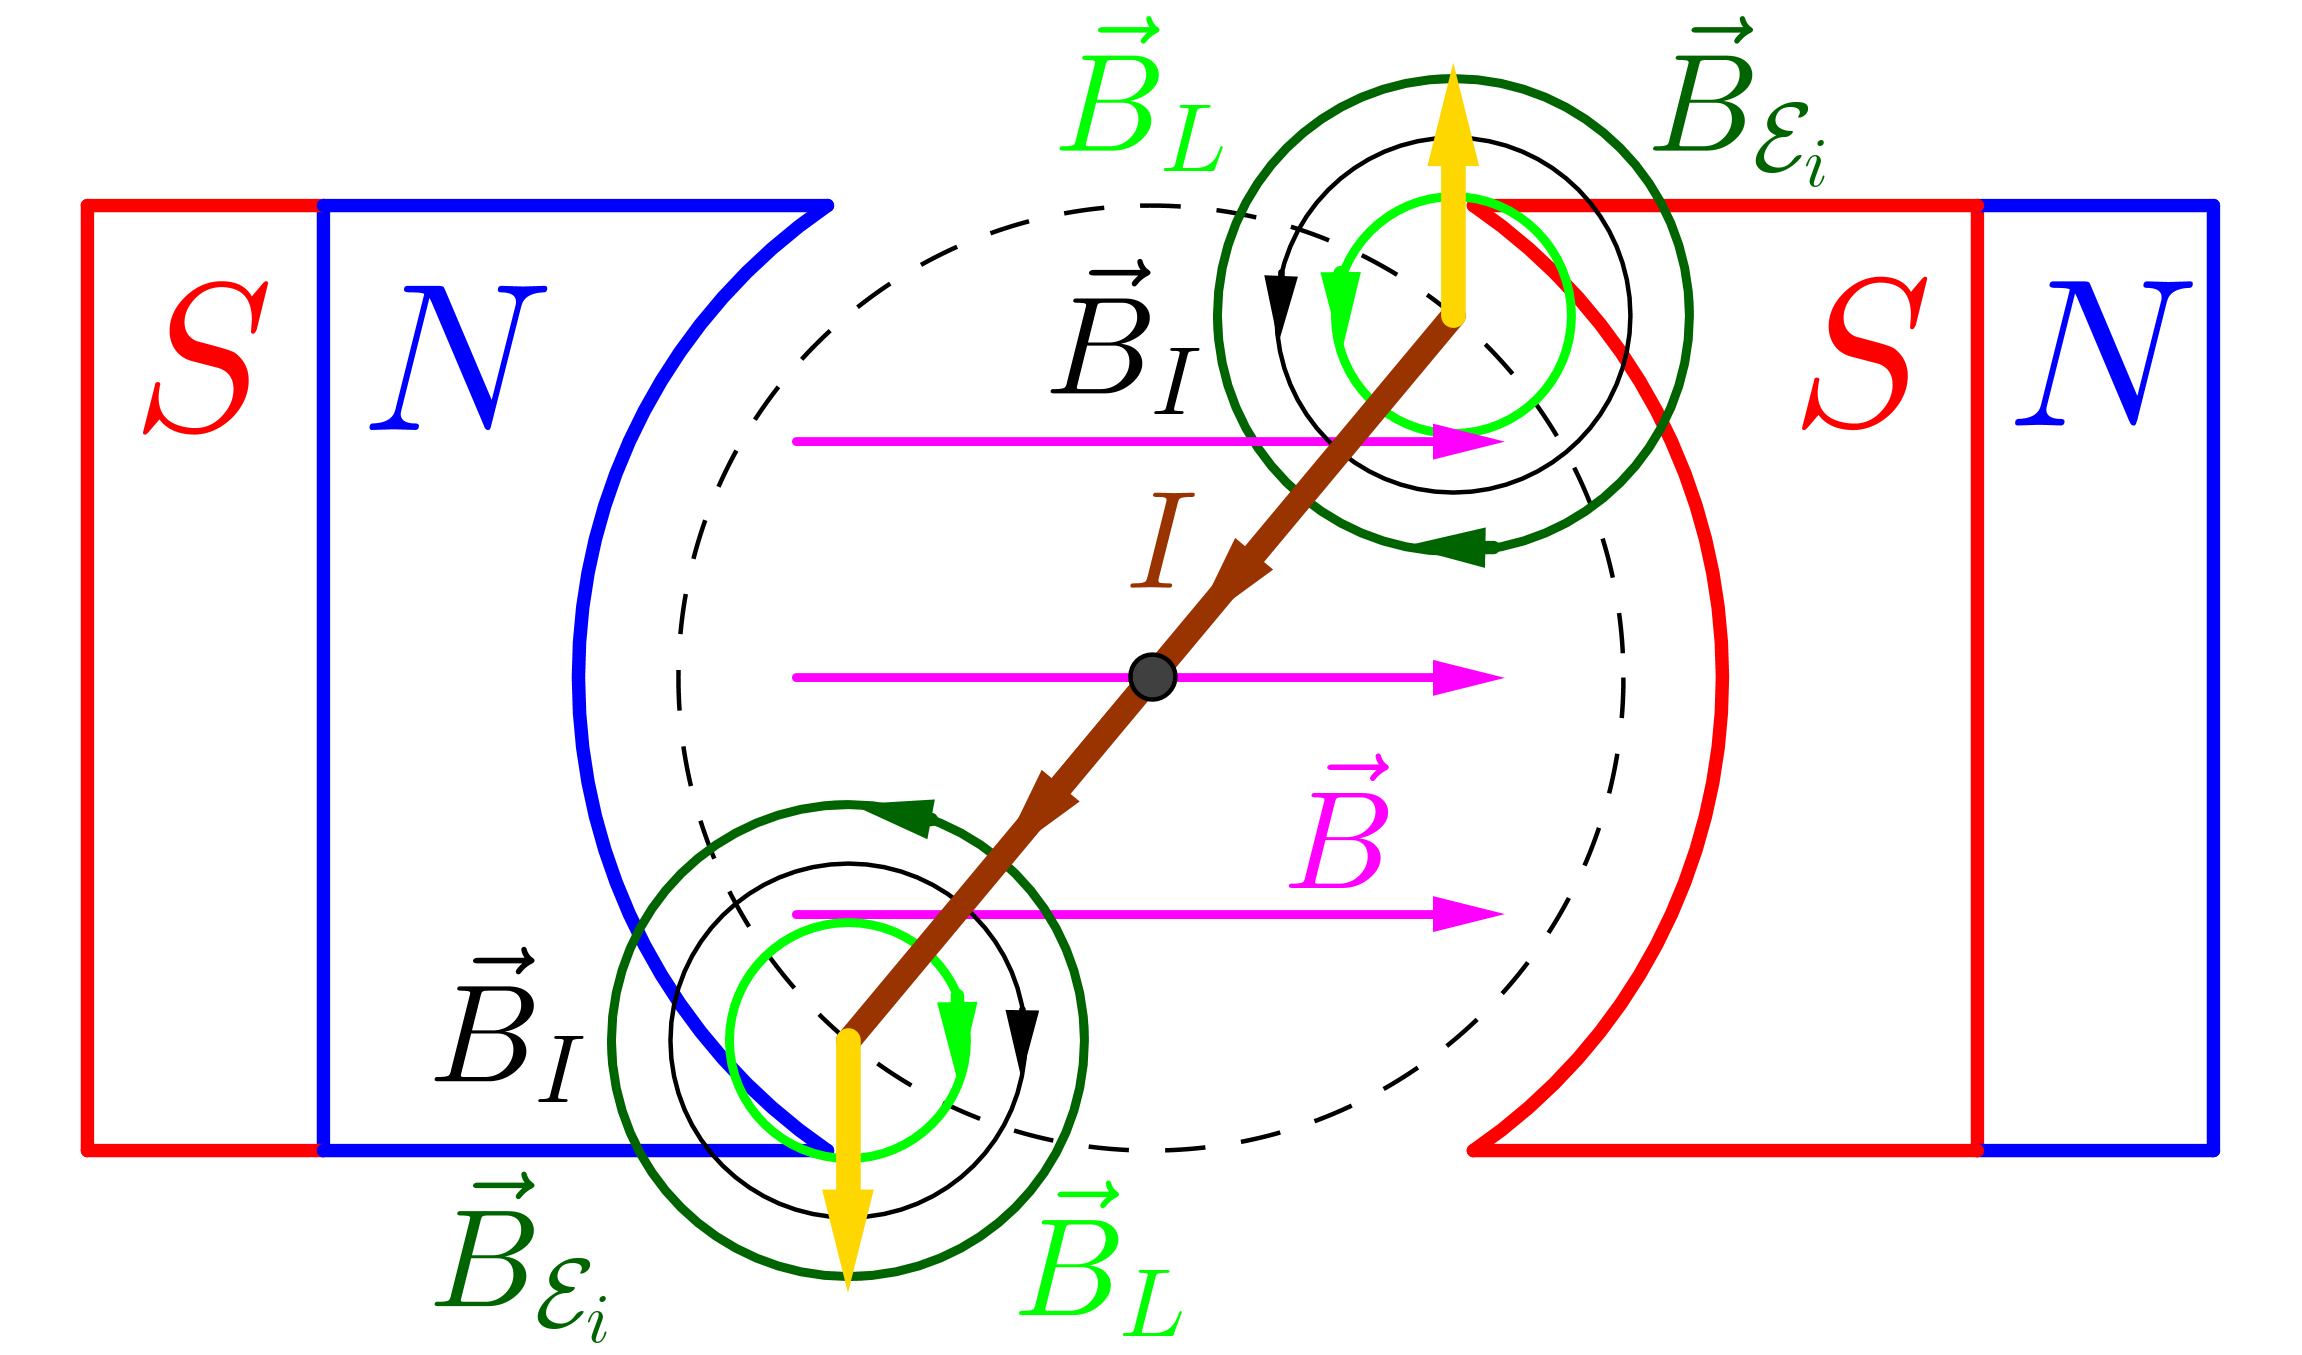
\includegraphics[height = 6cm]{pics/inductions.png}}
	\caption{Появление индукционных магнитных полей.}
	\label{inductions}
\end{figure}

Полный магнитный поток, пронизывающий контур, создается не только магнитным полем $\vec B$, но и магнитным полем $\vec B_I$, формируемым током в самом контуре.
Как мы уже сказали, появление ЭДС $\mathcal E_i$ приведет к тому, что ослабнет ток в контуре.
Это же, в свою очередь, приведет к ослаблению поля $\vec B_I$, а следовательно и к уменьшению создаваемого им магнитного потока, пронизывающего контур.
Последнее обстоятельство вызовет появление в контуре ЭДС самоиндукции $L_\textit{р}\dot I$, создающей дополнительный ток, направленный так, чтобы препятствовать ослаблению магнитного поля $\vec B_I$.
Для этого его магнитное поле $\vec B_L$ должно быть сонаправлено полю $\vec B_I$, а значит и данный индуцированный ток должен быть сонаправлен с током в самом контуре. 
Последнее говорит о том, что значение ЭДС самоиндукции должно складываться с ЭДС источника тока. 
Внимательно посмотрев теперь на уравнение~\eqref{Om's_law}, можно заметить, что оно говорит нам о том же: общий ток контура из-за действия ЭДС $\mathcal E_i$ уменьшается, следовательно производная $\dot I$ оказывается меньшей нуля, следовательно с учетом минуса, стоящего перед слагаемым $L\dot I$, это говорит о том, что соответствующая ЭДС $|L\dot I|$ суммируется с $U_{ctrl}$.

Вернемся к уравнениям.
Объединим несколько переписанные выражения~\eqref{from_lab_1} и \eqref{Om's_law} в систему
\begin{equation}\label{raw_system}
	\left\{	
		\begin{aligned}
			&\dot{\omega} = \frac{M_{el} + M_{oth}}{J}\\
			&\dot{I} =\frac{1}{L_\textit{р}}U_{ctrl} - \frac{1}{L_\textit{р}}\mathcal E_i - \frac{R}{L_\textit{р}}I\ldotp
		\end{aligned}
	\right.
\end{equation}
Заметим, что в полученном виде она представляет из себя лишь два независимых дифференциальных уравнения относительно функций $\omega(t)$ и $I(t)$. 
Также заметим, что представленные уравнения содержат функции $M_{el}$ и $\mathcal E_i$, вид которых на данном этапе нельзя установить ни через выходные сигналы, ни через выходные.
Все сказанное свидетельствует о том, что система~\eqref{raw_system} также подлежит уточнению и пока что не может претендовать на роль математической модели.

Для того чтобы найти связь между составляющими полученную систему уравнениями и одновременно установить зависимости величин $M_{el}$ и $\mathcal E_i$ от других функций и параметров, входящих в эти уравнения, получим на основании физики процесса два равенства, выполняющиеся для двигателей постоянного тока.
Все объяснения будем давать на примере ранее введенной модели двигателя.

Во-первых,  выясним, как возникает раскручивающий якорь момент силы $M_{el}$.
Несложно догадаться, что он создается действующими на стороны контура силами Ампера (рис.~\ref{Mel}) и, следовательно, равен
\begin{equation}
	M_{el} = 2F_\text{А}r_x,
\end{equation}   
где $r_x=r_\text{к}\cos\gamma$~--- плечо силы $\vec F_\text{А}$.
Раскрыв силу Ампера по соответствующей формуле, можно получить следующее выражение:
\begin{equation}\label{bad_for_km}
	M_{el} = 2(BIl_\text{к})r_x,
\end{equation}
где $l_\text{к}$~--- длина сторон\footnote{Заметим, что они перпендикулярны силовым линиям магнитного поля $\vec B$. Именно по этой причине при написании выражения для $F_\text{А}$ был опущен синус ($\sin 90^\circ = 1$).} контура, на которые действуют силы Ампера, раскручивающие ротор (рис.~\ref{rotor_in_model}).
Введя обозначение 
\begin{equation}\label{constr_const_km}
	k_m = 2Bl_\text{к}r_x,
\end{equation}
перепишем уравнение~\eqref{bad_for_km} в виде
\begin{equation}\label{for_km}
	M_{el} = k_mI\ldotp
\end{equation}

\begin{figure}[h]
	\begin{center}
		\begin{minipage}[h]{0.49\linewidth}
			\centering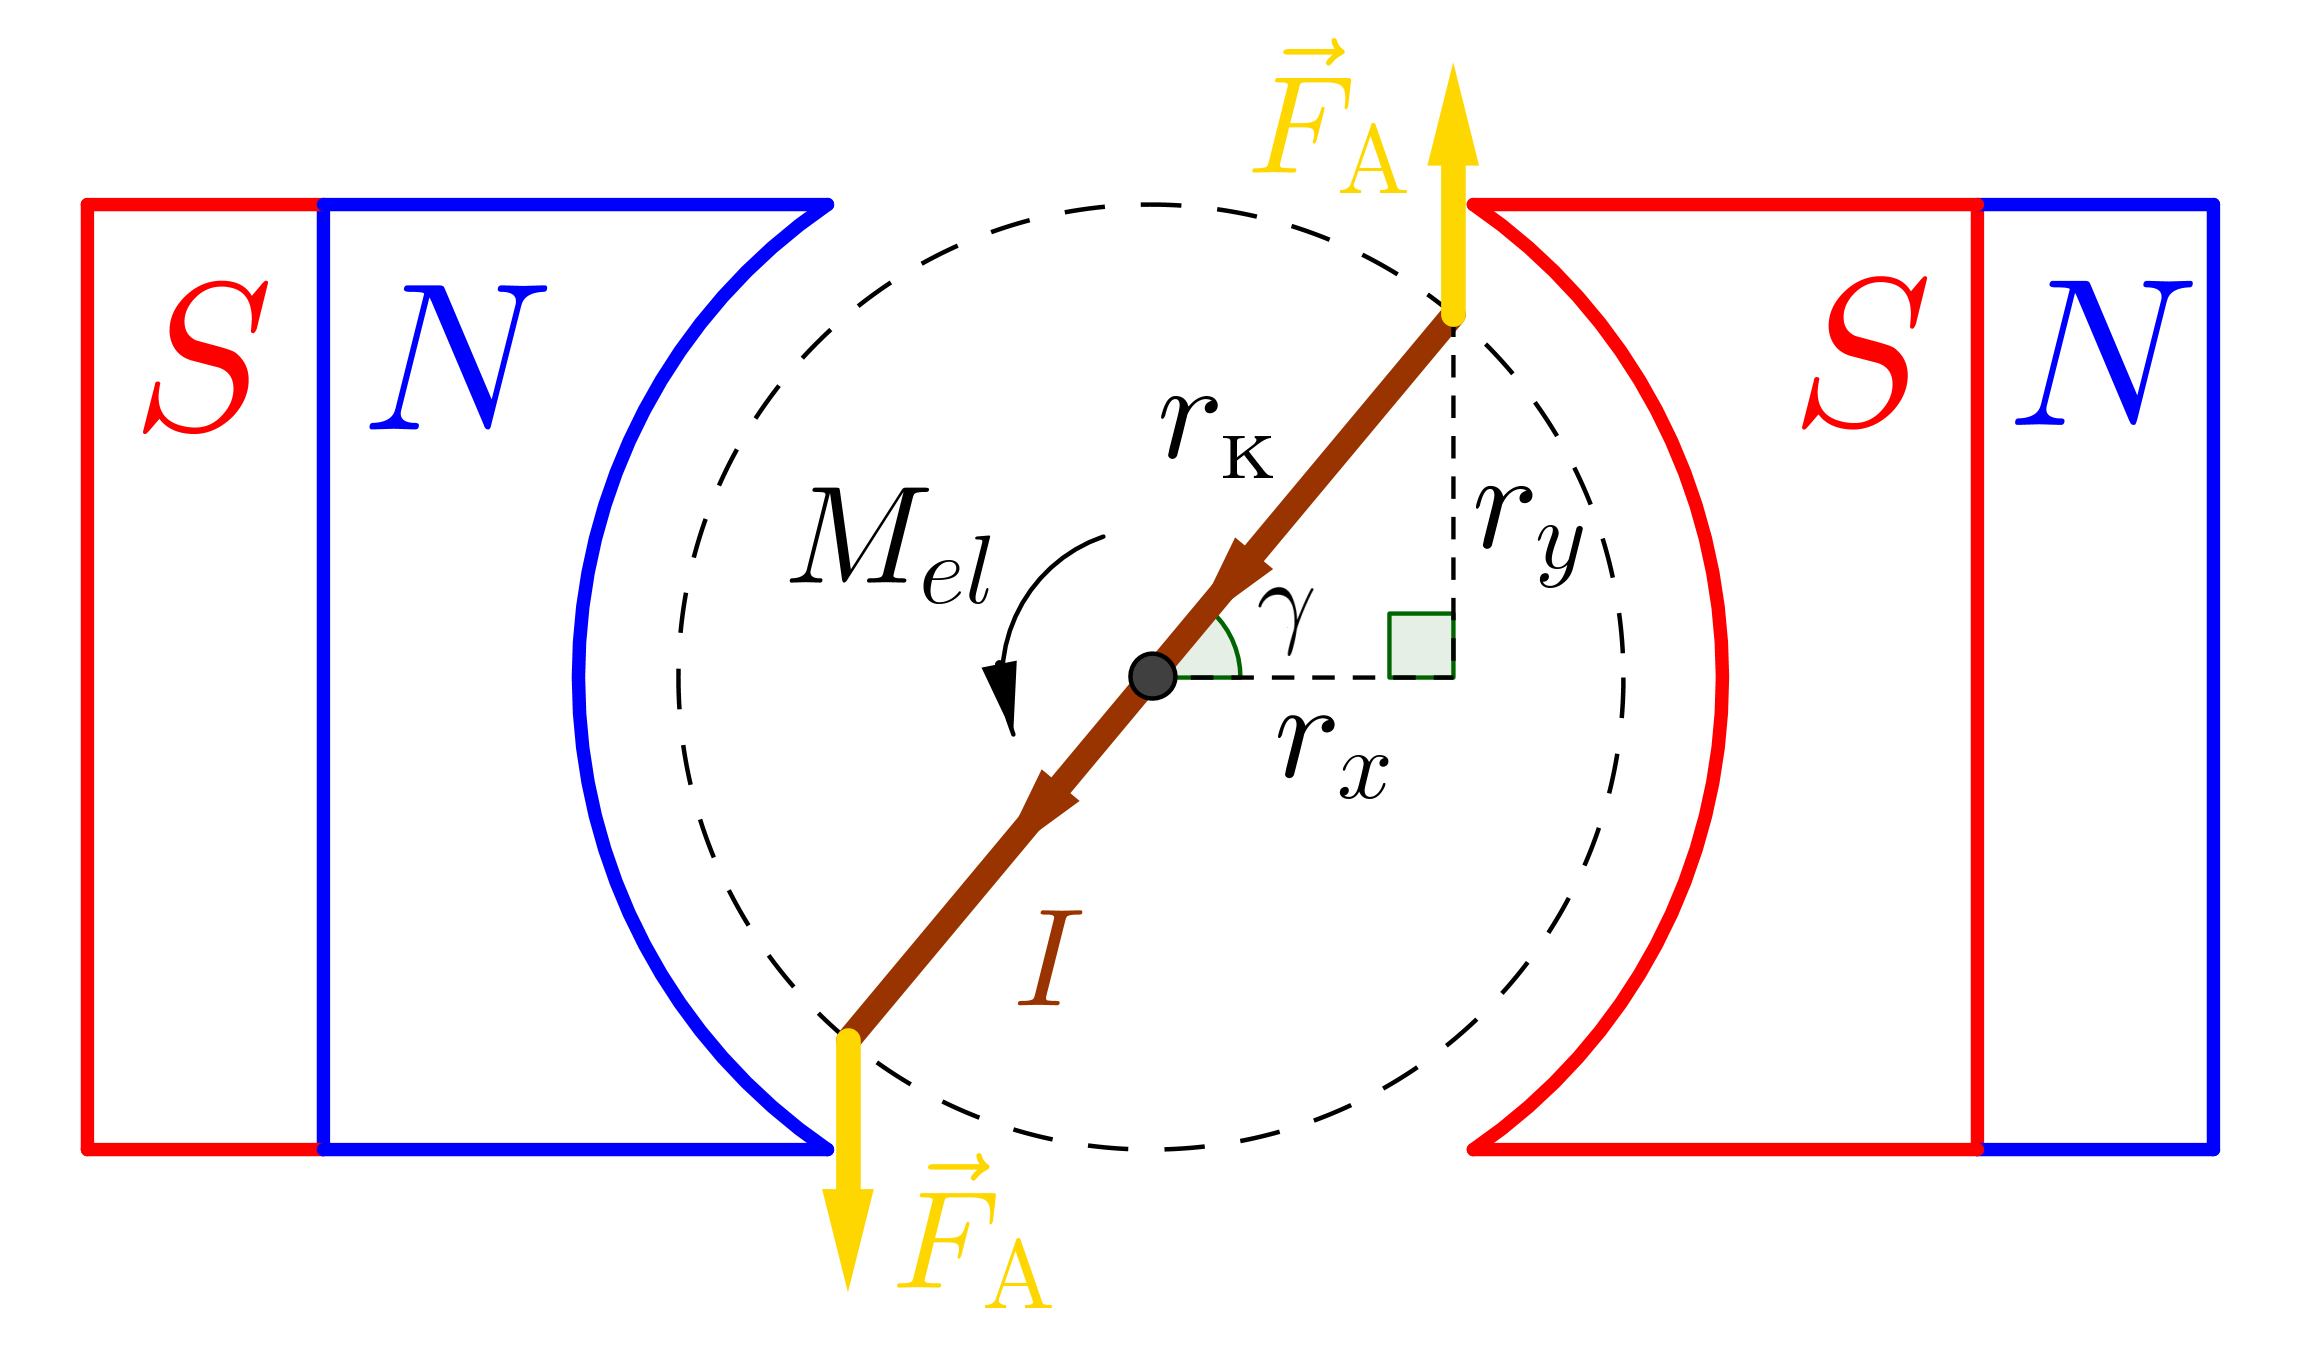
\includegraphics[height=5cm]{pics/Mel.png}
			\caption{Возникновение момента $M_{el}$.}
			\label{Mel} 
		\end{minipage}
		\hfill 
		\begin{minipage}[h]{0.49\linewidth}
			\centering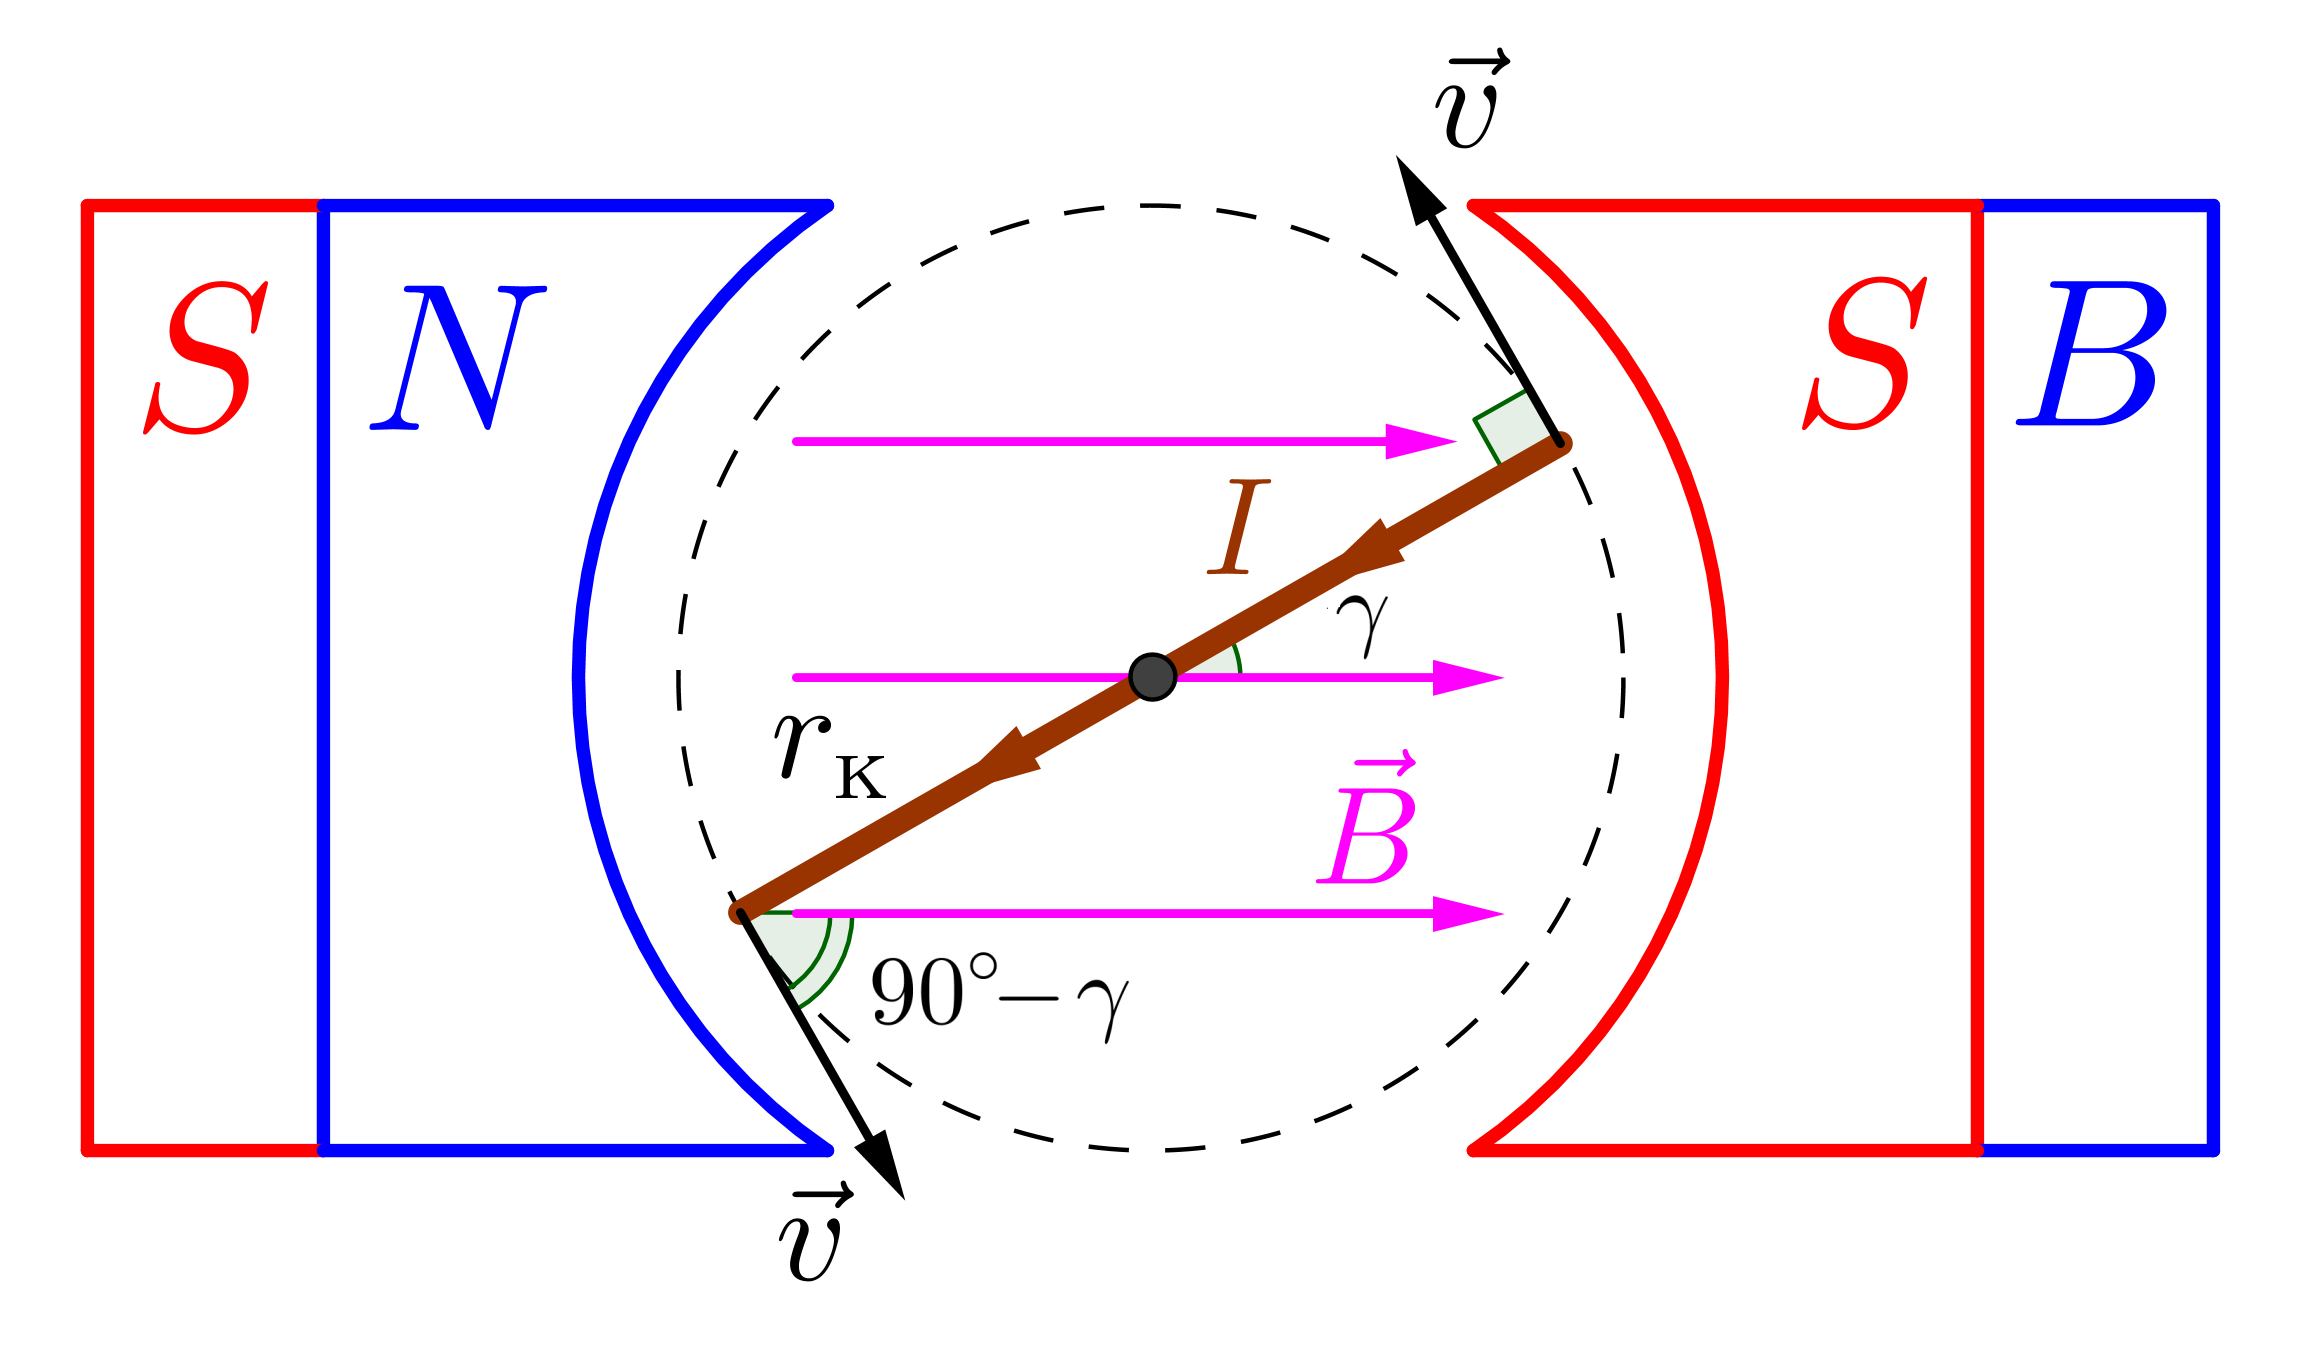
\includegraphics[height=5cm]{pics/Ei.png}
			\caption{Появление ЭДС $\mathcal E_i$.}
			\label{Ei}
		\end{minipage}
	\end{center}
\end{figure}

Во-вторых, получим выражение для ЭДС индукции $\mathcal E_i$.
Как известно еще из школьного курса физики, в проводнике, движущемся в магнитном поле, наводится некоторая ЭДС индукции, прямопропорциональная значению магнитной индукции окружающего его поля, длине проводника и скорости его движения. 
Следовательно, в проводниках, составляющих контур якоря, также должна индуцироваться данная ЭДС.
По правилу левой руки можно установить, что в сторонах контура, имеющих длину $2r_\text{к}$, она оказывается перпендикулярной им, а значит на ток в контуре никак не влияет.
В~двух других же сторонах, значения длин которых равны $l_\text{к}$, эта ЭДС действует вдоль проводников противоположно протекающему в контуре току\lefteqn.\footnote{Заметим, что данное утверждение является альтернативным предложенному ранее обоснованием постановки минуса перед $\mathcal E_i$ в формуле~\eqref{Om's_law}.}

Применяя соответствующую формулу, получим для $\mathcal E_i$ следующее выражение:
\begin{equation}
	\mathcal E_i = 2Bl_\text{к}v\sin(90^\circ-\gamma) = 2Bl_\text{к}v\cos\gamma,
\end{equation}
где $v$~--- линейная скорость вращения соответствующих сторон контура (рис.~\ref{Ei}), а множитель $2$ поставлен из-за того, что одинаковая ЭДС, равная $Blv\cos\gamma$, индуцируется одновременно в обеих сторонах контура, имеющих длину $l_\text{к}$. 
Выразив линейную скорость вращения ротора через угловую, получим
\begin{equation}
	\mathcal E_i = 2Bl_\text{к}\omega r_\text{к}\cos\gamma = 2Bl_\text{к}\omega r_x.
\end{equation}
Введя же обозначение 
\begin{equation}\label{constr_const_ke}
	k_e = 2Bl_\text{к}r_x,
\end{equation}
окончательно будем иметь\footnote{Можно заметить, что это уравнение мы уже использовали в первой лабораторной работе. Единственное, в ней мы обозначили постоянную $k_e$ через $\alpha_2$.}
\begin{equation}\label{for_ke}
	\mathcal E_i = k_e\omega\ldotp
\end{equation}

Заметим, что входящие в эти уравнения величины $k_m$ и $k_e$ равны ($ k_m=k_e=k$)\lefteqn{.}\footnote{Вопреки этому, в данном курсе мы будем рассматривать их как две самостоятельные величины.}
Также заметим, что, строго говоря, $k$ не является постоянной величиной, потому что входящее в определяющее ее выражение плечо силы Ампера $r_x$ зависит от угла поворота ротора.
Несмотря на это, устройство настоящих двигателей постоянного тока и непрерывное вращение якоря, приводящее к тому, что значение угла $\gamma$ постоянно меняется, а следовательно приходится работать с некоторым средним его значением, создают такие условия, в которых $k$ является (рассматривается) постоянной величиной и называется \textit{конструктивной постоянной двигателя}.
При этом, согласно уравнениям~\eqref{for_km} и \eqref{for_ke}, зависимости $M_{el}$ от $I$ и $\mathcal E_i$ от $\omega$ получаются линейными.

Вернемся к математической модели.
Подставив равенства~\eqref{for_km} и~\eqref{for_ke} в систему~\eqref{raw_system}, получим
\begin{equation}\label{the_main_system}
	\left\{	
		\begin{aligned}
			&\dot{\omega} = \frac{k_m}{J}I + \frac{M_{oth}}{J}\\
			&\dot{I} =\frac{1}{L_\textit{р}}U_{ctrl} - \frac{k_e}{L_\textit{р}}\omega - \frac{R}{L_\textit{р}}I
		\end{aligned}
	\right.
\end{equation}
Данная система уравнений при условии, что известны зависимости $U_{ctrl}(t)$ и $M_{oth}(t)$ (входные сигналы), может быть решена относительно функций $\omega(t)$ и $I(t)$ (выходные сигналы). 
Этот факт показывает, что она является искомой математической моделью работы электродвигателя: с её помощью можно установить, как он будет вести себя в той или иной ситуации. 

Например, для случая работы ненагруженного двигателя ($M_{oth} = 0$) от источника постоянного напряжения ($U_{ctrl}(t) = const$), который мы  рассматривали в первой работе, из этой системы получаются следующие выражения для $\omega(t)$ и $I(t)$:
\begin{gather}\label{w(t)}
	\omega(t) = C_1\exp\left(\varkappa_1t + \varkappa_2t\right) +C_2\exp\left(\varkappa_1t-\varkappa_2 t\right)+\frac{U_{ctrl}}{k_e},\\
	I(t) = C_3\exp\left(\varkappa_1t + \varkappa_2t\right) - C_3\exp\left(\varkappa_1t - \varkappa_2t\right),\label{I(t)}
\end{gather}
где
\begin{equation}
	C_1 = \frac{U_{ctrl}}{2k_e}\left(\frac{\varkappa_1}{\varkappa_2} - 1\right),
\end{equation}
\begin{equation}
	C_2 = -\frac{U_{ctrl}}{2k_e}\left(\frac{\varkappa_1}{\varkappa_2} + 1\right),
\end{equation}
\begin{equation}
	C_3 = \frac{J}{k_m}\cdot\frac{U_{ctrl}}{2k_e}\left(\frac{\varkappa_1^2}{\varkappa_2} - \varkappa_2\right)\!\!,
\end{equation}
где, в свою очередь,
\begin{equation}
	\varkappa_1 = -\frac{R}{2L_\textit{р}},
\end{equation}
\begin{equation}
	\varkappa_2 = \sqrt{\varkappa_1^2 - \frac{k_mk_e}{JL_\textit{р}}},
\end{equation}

Графики, полученные с помощью представленных уравнений при небольших значениях индуктивности, имеют вид, показанный на рис.~\ref{graph_w(t)} и \ref{graph_I(t)}.
Из них в первую очередь вытекают следующие факты.

\begin{figure}[h]
	\noindent\centering{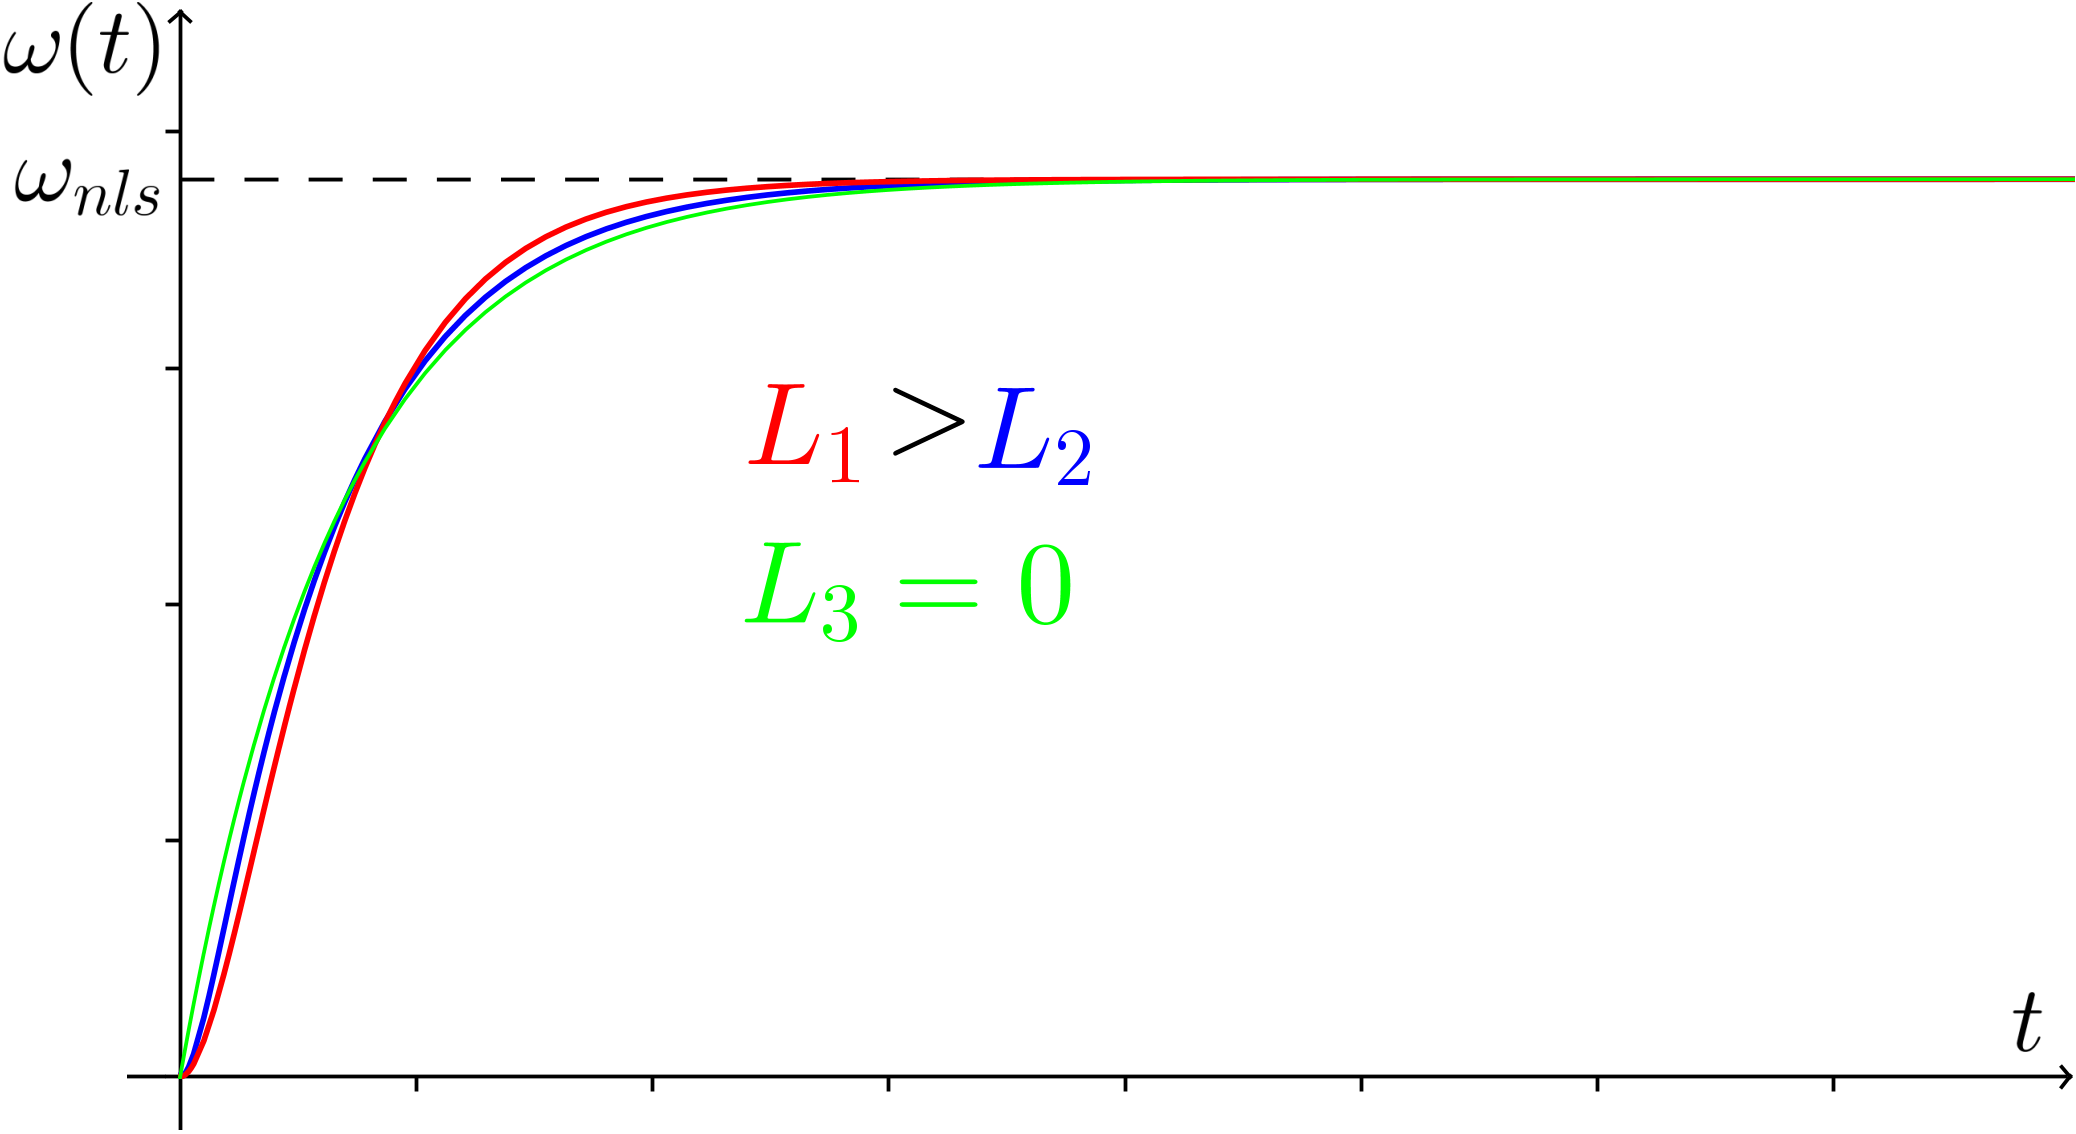
\includegraphics[scale=1.5]{pics/graph_w(t).png}}
	\caption{График зависимости угловой скорости вращения ротора от времени.}
	\label{graph_w(t)}
\end{figure}

Во-первых, графики с рис.~\ref{graph_I(t)} показывают, что при установлении постоянной скорости вращения ротора сила тока в его обмотке обращается в нуль.
Согласно уравнению~\eqref{for_km}, это означает, что в нуль обращается и вращательный момент $M_{el}$.
Как мы уже говорили в первой работе, данная особенность подтверждается опытами.
Во-вторых, все те же графики говорят нам о том, что вращательный момент $M_{el}$ достигает своего максимального значения тем дольше, чем больше индуктивность обмотки якоря.
При этом по мере роста $L_\textit{р}$ максимальное значение $M_{el}$ уменьшается.
Относительно быстроты достижения скоростью вращения ротора $\omega$ своего максимального значения $\omega_{nls}$ наблюдается обратная зависимость: с возрастанием $L_\textit{р}$ функция $\omega(t)$ стремится к значению $\omega_{nls}$ все быстрее.

\begin{figure}[h]
	\noindent\centering{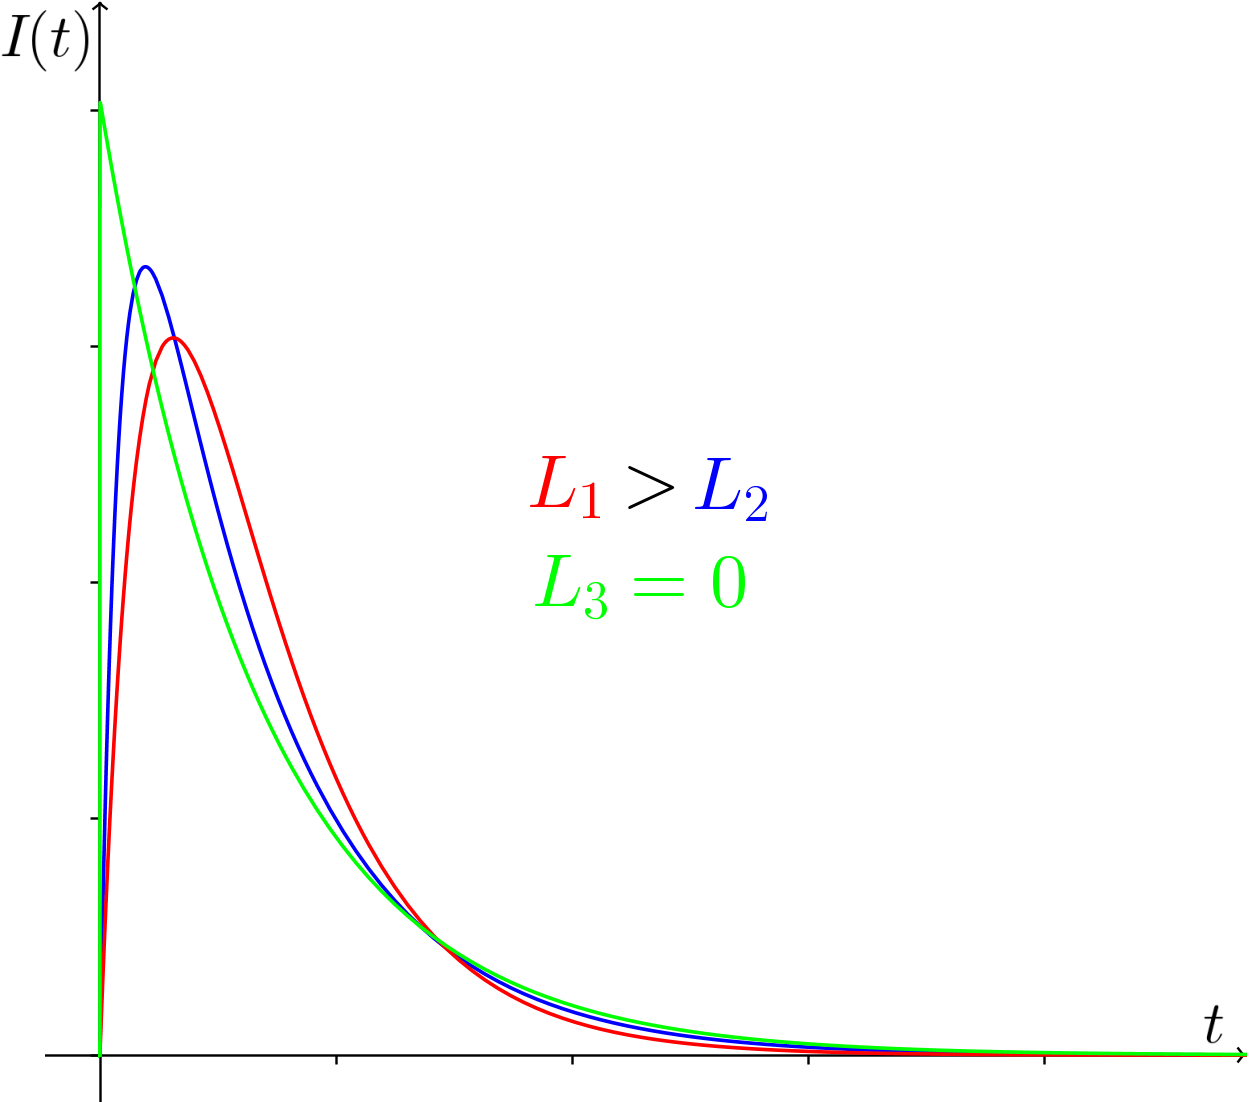
\includegraphics[scale=2]{pics/graph_I(t).png}}
	\caption{График зависимости силы тока ротора от времени.}
	\label{graph_I(t)}
\end{figure}

Важно отметить то, что графики на рис.~\ref{graph_w(t)} зрительно схожи с тем, который мы получили для функции $\omega(t)$ в первой работе. 
Такое согласие, несмотря на то, что в первой работе при составлении математической модели мы предположили момент $M_{el}$ пропорциональным полному напряжению в цепи, а не силе тока, как должно быть на самом деле, и пренебрегли при нахождении полного напряжения в цепи слагаемым $L_\textit{р}\dot I$ (или, что то же самое, положили $L_\textit{р} = 0$), можно объяснить, если обратиться к той особенности для представленных графиков, о которой мы уже упоминали~--- они были построены для небольших значений индуктивности.
Учитывая указанное свойство, согласно уравнению~\eqref{Om's_law}, получаем, что в таком случае при проведении математических выкладок можно пренебречь последним слагаемым в его левой части.
В~результате этого действия получится, что сила тока будет пропорциональна полному напряжению в цепи. 
Из последнего факта, в свою очередь, следует, что момент силы также будет пропорционален напряжению.
Как видно, мы пришли к тем заключениям, которыми руководствовались в первой работе.

Сказанное позволяет сделать вывод о том, что рассмотренная нами в прошлой лабораторной математическая модель работы двигателя является частным случаем системы~\eqref{the_main_system} при $L_\textit{р}=0$.
Проверим это~--- положим в системе~\eqref{the_main_system} $L_\textit{р}=0$ и решим получившиеся дифференциальные уравнения (или просто найдем выражения, в которые переходят уравнения~\eqref{w(t)} и \eqref{I(t)} при стремлении $L_\textit{р}$ к нулю). 
В результате получим
\begin{gather}\label{electro_w(t)}
	\omega(t) = \frac{U_{ctrl}}{k_e}\biggl(1-\exp\Bigl(-\frac{k_mk_e}{JR}\,t\Bigr)\biggr),\\
	I(t) = \frac{U_{ctrl}}{R}\exp\Bigl(-\frac{k_mk_e}{JR}\,t\Bigr)\ldotp \label{electro_I(t)}
\end{gather}
Легко видеть, что выражение~\eqref{electro_w(t)} для зависимости $\omega(t)$ совпадет с тем, которое было получено в прошлой работе, если окажутся справедливыми равенства
\begin{gather}\label{wo}
	\omega_{nls} = \frac{U_{ctrl}}{k_e},\\
	T_m = \frac{JR}{k_mk_e}\ldotp \label{Tm}
\end{gather}

Докажем их.

Рассмотрим величину $k_e$.
Согласно уравнению~\eqref{for_ke}, она равна:
\begin{equation}
	k_e = \frac{\mathcal E_i(t)}{\omega(t)}\ldotp
\end{equation}
Найдем значение функции $\mathcal E_i(t)$, соответствующее тому времени, когда функция $\omega(t)$ уже достигла своего максимального значения $\omega_{nls}$.
Как уже было сказано выше, при исследуемом режиме работы двигателя с достижением ротором своей постоянной скорости вращения сила тока в его обмотках становится постоянной и равной нулю.
Согласно этому, из уравнения~\eqref{Om's_law} следует, что при этом будет выполняться равенство
\begin{equation}\label{voltages}
	\mathcal E_i = U_{ctrl}.
\end{equation}
С~учетом всего сказанного имеем, что $k_e$ можно определить из выражения
\begin{equation}\label{ke}
	k_e = \frac{U_{ctrl}}{\omega_{nls}},
\end{equation}
которое и доказывает справедливость уравнения~\eqref{wo}.

Идем дальше.
В~прошлой работе было сказано, что пусковой момент двигателя $M_{st}$ является максимальным значением момента $M_{el}$ и достигается в начальный момент времени $t=0$.
В~данной работе мы показали, что вращательный момент $M_{el}$ прямопропорционален силе тока в обмотке якоря.
Несколькими абзацами выше для силы тока в цепи разгоняющегося ненагруженного двигателя было получено выражение~\eqref{electro_I(t)}.
Из него в полном согласии со сказанным про функцию $M_{el}(t)$ следует, что сила тока также максимальна в начальный момент времени, а потом монотонно убывает, в конце концов обращаясь в нуль.  
Следовательно, для величины $M_{st}$ оказывается справедливой формула
\begin{equation}\label{Mst}
	M_{st} = k_mI(0) = \frac{k_mU_{ctrl}}{R}\ldotp
\end{equation}

Согласно материалам прошлой работы, для электромеханической постоянной времени имеем
\begin{equation}
	T_m = \frac{J\omega_{nsl}}{M_{st}}\ldotp
\end{equation}
Сделав в данном уравнении подстановки, согласно выражениям~\eqref{wo} и \eqref{Mst}, получим для $T_m$ выражение~\eqref{Tm}:
\begin{equation}
	T_m = \frac{J\omega_{nsl}}{M_{st}} \stackrel{\eqref{wo}}{=} \frac{JU_{ctrl}}{M_{st}k_e} \stackrel{\eqref{Mst}}{=}
	\frac{JR}{k_mk_e}\ldotp
\end{equation}

Таким образом, мы показали, что рассмотренная нами в первой лабораторной математическая модель двигателя является частным случаем ее версии, выведенной в данной работе.
Хорошее совпадение с результатами эксперимента в прошлой работе объясняется тем, что индуктивность двигателя EV3 и есть очень маленькая величина.
Ее значение составляет приблизительно $\text{0.0047 Гн}$.

\paragraph*{Схема моделирования}$\phantom{-}$\\
\hspace*{\parindent}Схема моделирования процесса разгона ненагруженного ротора двигателя, согласно системе уравнений~\eqref{the_main_system}, примет вид, показанный на рис.~\ref{struct_sheme}.
По сравнению со схемой, использованной в первой лабораторной, эта ничего принципиально нового в себе не несет. 
Единственное отличие, которое все же имеется, заключается в том, что используются сразу два блока с надписью <<To workspace>> для записи получаемых данных: нижний из них нужен для фиксации значений угловой скорости, а второй (верхний)~--- значений силы тока. 

\begin{figure}[h]
	\noindent\centering{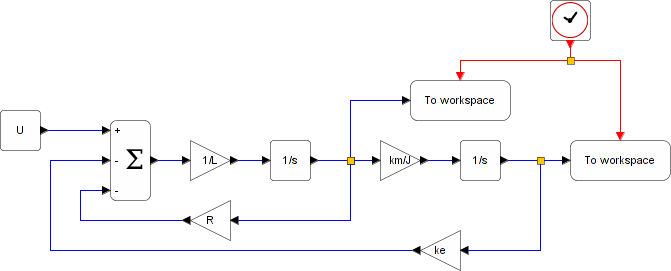
\includegraphics[scale=0.9]{pics/struct_sheme.png}}
	\caption{Схема моделирования процесса разгона ненагруженного двигателя.}
	\label{struct_sheme}
\end{figure}

В~заключении данного раздела упомянем о следующем.

Как уже было сказано, любой процесс характеризуется входными и выходными сигналами, а также функциональной зависимостью между ними. 
При этом, если мы будем рассматривать разные процессы, происходящие в одной и той же системе (в одном и том же объекте), они будут описываться только разными входными и выходными сигналами, функциональная же зависимость между ними меняться не будет.
Если первое достаточно очевидно, то второе следует пояснить хотя бы рассмотренным примером: при составлении уравнений для математической модели двигателя мы не учитывали вид входных и выходных сигналов ($U_{ctrl}$, $M_{oth}$ и $\omega$, $I$ соответственно), следовательно полученные уравнения, играющие роль функциональной связи, оказываются справедливыми независимо от того, как выглядят упомянутые функции.

Если указанное свойство не дает особых преимуществ при исследовании процессов путем решения дифференциальных уравнений (все равно их придется решать), то в случае со  схемами моделирования оно приводит к значительному упрощению.
Заключается последнее в том, что схемы разных процессов, происходящих в одном и том же объекте (в одной и той же системе), имеют в своем составе общую, неизменяемую часть.
В~связи с этим можно сказать, что последняя характеризует сам исследуемый объект, а не только какой-то конкретный процесс.
При этом, чтобы перейти от рассмотрения одного процесса, протекающего в данной системе, к другому, достаточно только поменять блоки, ответственные за входные и выходные сигналы.

\begin{figure}[h]
	\noindent\centering{ 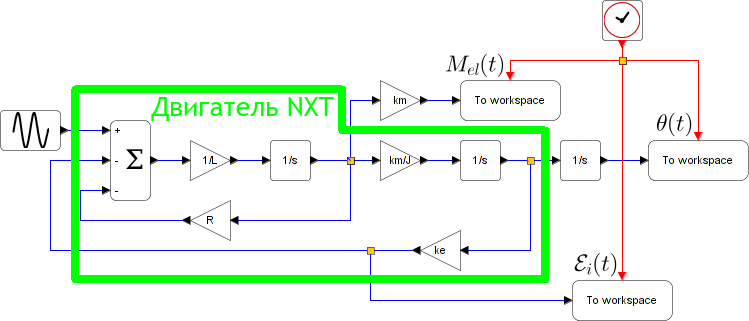
\includegraphics[scale=0.9]{pics/struct_sheme_for_sin.png} }
	\caption{Схема моделирования работы двигателя при его подключении к источнику переменного напряжения.}
	\label{struct_sheme_for_sin}
\end{figure}

Покажем сказанное на примере.
Для этого обратимся к рис.~\ref{struct_sheme_for_sin}; на нем показана схема, которую придется составить, когда мы захотим исследовать поведение ненагруженного двигателя при подаче на него синусоидального напряжения.
При этом пусть нас будут интересовать в качестве выходных сигналов не функции $\omega(t)$ и $I(t)$, а зависимости $M_{el}(t)$, $\theta(t)$ и $\mathcal E_i(t)$.
Сравнивая ее и схему на рис.~\ref{struct_sheme}, находим подтверждение нашим словам: они действительно отличаются только блоками, отвечающими за входные (управляющие) воздействия и выходные сигналы, и обе содержат постоянную часть~--- схему исследуемого электродвигателя постоянного тока (обведена зеленой рамкой).

\paragraph*{Дополнительные сведения}$\phantom{-}$\\
\hspace*{\parindent}То, что до этого времени мы называли двигателем EV3, на самом деле представляет из себя некоторое более сложное устройство, в котором обычный электродвигатель играет роль всего лишь одной из его частей.
Например, помимо последнего мотор EV3 содержит \textit{редуктор}~--- систему шестерней, соединяющих его внешний вал с валом находящегося внутри него электродвигателя, датчик, измеряющий угол поворота внешнего вала, и некоторую микросхему (рис.~\ref{motor_inside}).

\begin{figure}[h]
	\center{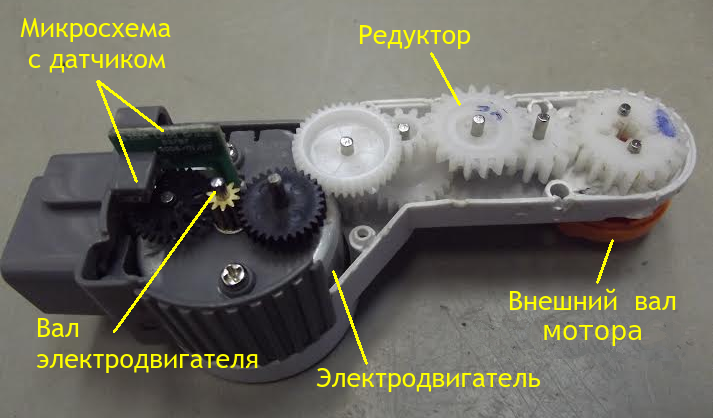
\includegraphics[scale = 0.6]{pics/motor_inside.png}}
	\caption{Мотор EV3.}
	\label{motor_inside}
\end{figure}

Несложно догадаться, что в этом случае все уравнения, полученные выше для обычного двигателя, без определенных изменений не будут справедливы для мотора EV3.
Дело в том, что в этом случае, как минимум, встает вопрос о его моменте инерции $J$: что под ним понимать?
Рассматривая мотор EV3 мы интересуемся поведением (например, видом функций $M_{el}(t)$ и $\omega(t)$) только его внешнего вала.
Однако, очевидно, что момент инерции последнего в чистом виде не будет искомым $J$.
Чтобы разобраться с указанной проблемой скажем следующее.

Предположим, что редуктор мотора EV3 содержит всего три шестерни~--- см.~рис.~\ref{gears}\lefteqn.\footnote{Для большего числа шестерней и других способов их сопряжения все выкладки, которые мы получим в дальнейшем, выводятся аналогично.}
Будем считать, что ведущей является шестерня~№1 (она будет служить моделью вала электродвигателя), а ведомой, следовательно, шестерня~№3 (она будет служить моделью внешнего вала мотора EV3).

\begin{figure}[h]
	\center{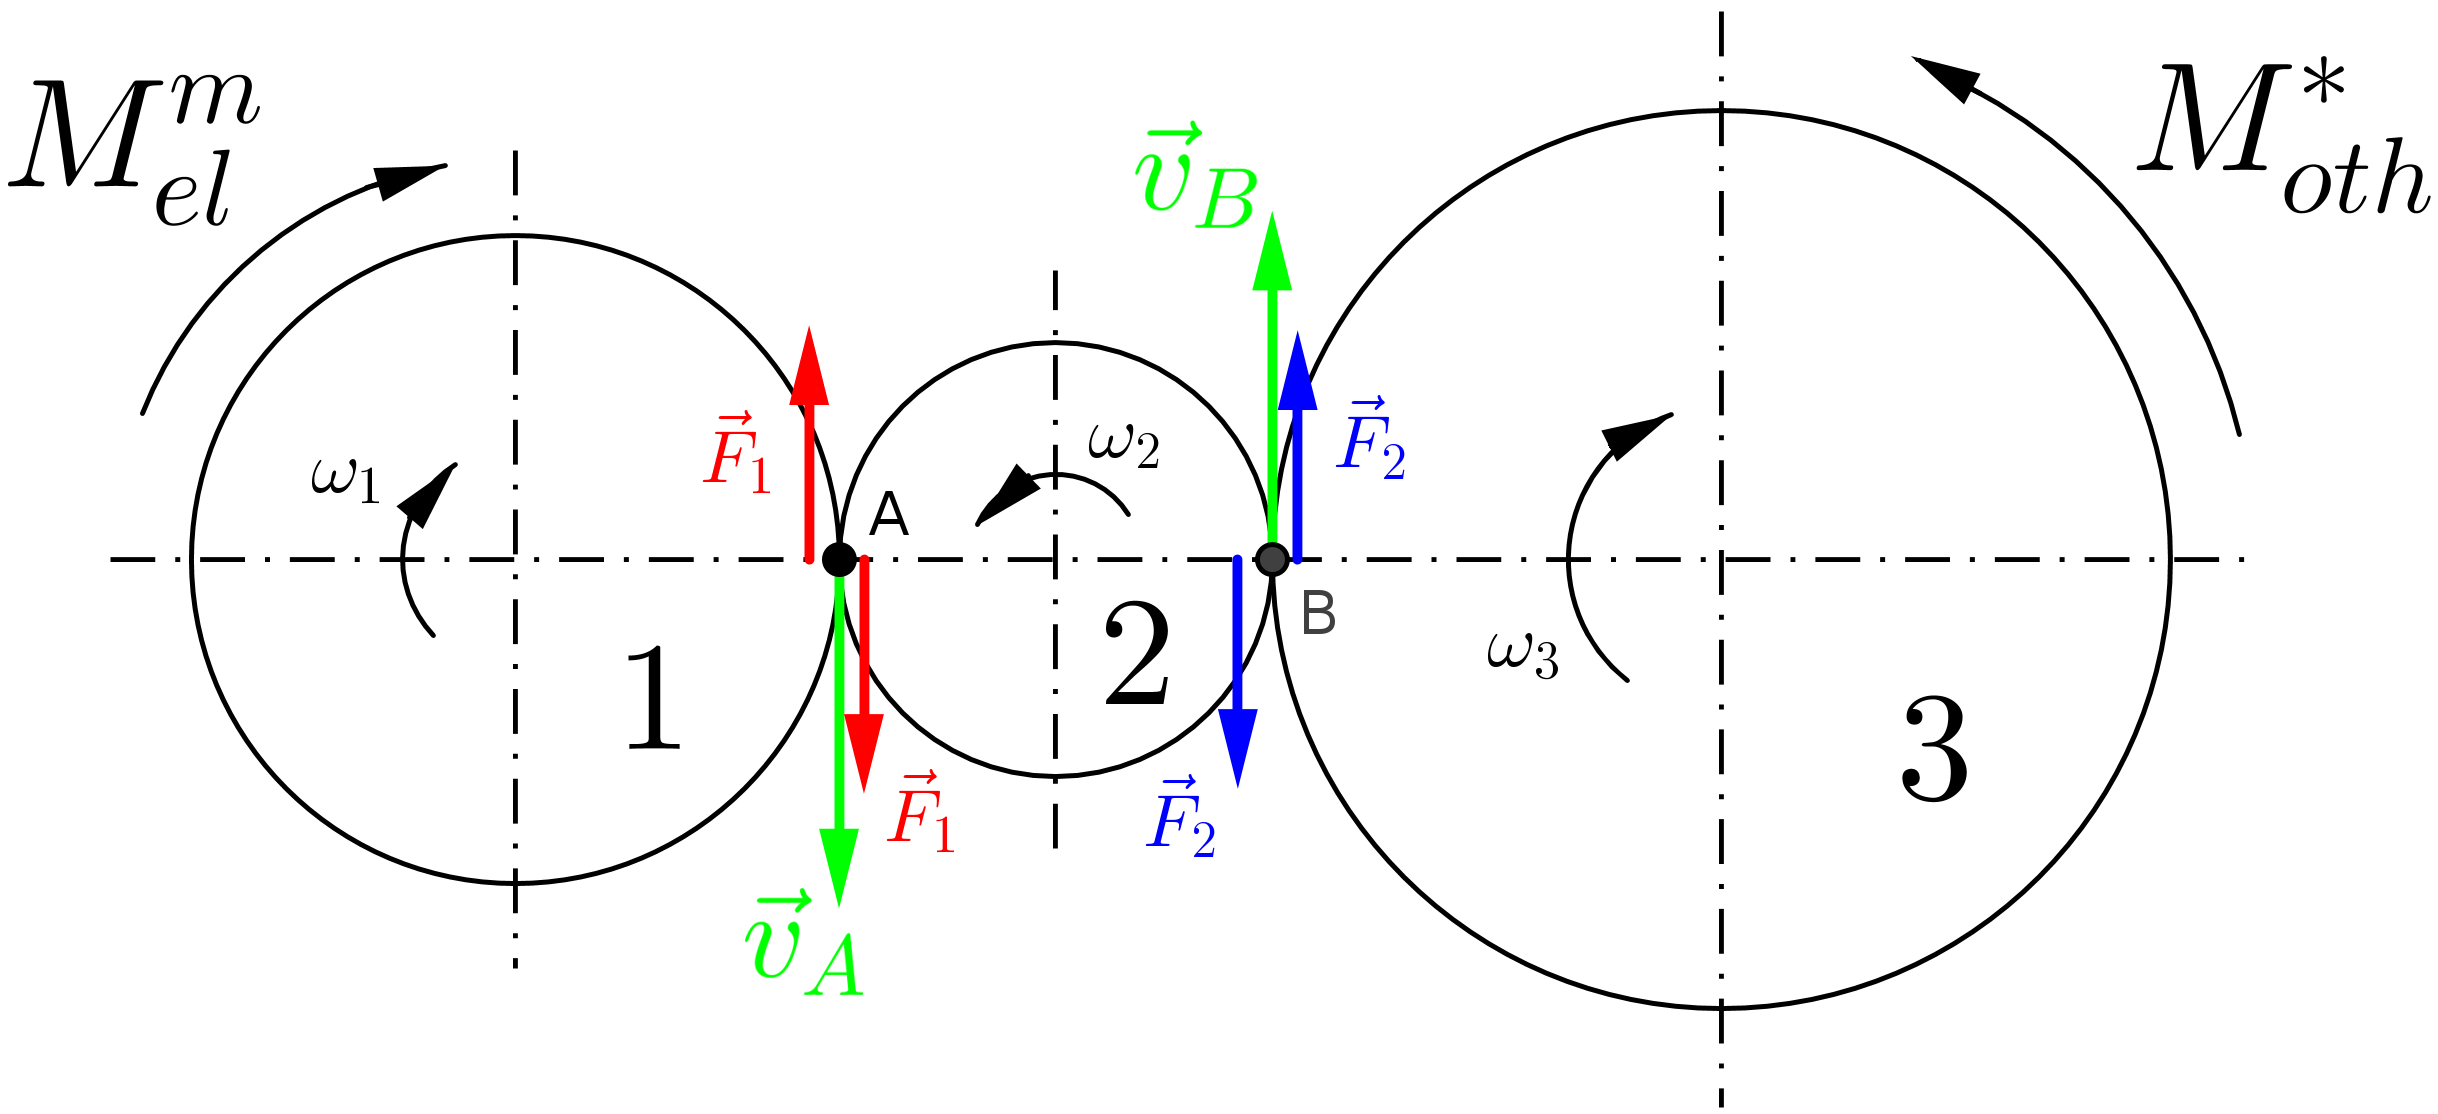
\includegraphics[scale = 1.2]{pics/gears.png}}
	\caption{Модель мотора.}
	\label{gears}
\end{figure}

Запишем для шестерней (в рассматриваемой модели~--- соприкасающихся без проскальзывания цилиндров) уравнения второго закона Ньютона:
\begin{gather}
	M_{el}^{m} - F_1r_1 = J_1\dot\omega_1,\\
	F_1r_2 - F_2r_2 = J_2\dot\omega_2,\\
	F_2r_3 - M_{oth}^* = J_3\dot\omega_3,
\end{gather}
где $J_i$, $r_i$ и $\omega_i$~--- момент инерции, радиус и угловая скорость вращения шестерни №$i$ соответственно; $M_{el}^{m}$~--- момент силы, раскручивающий первую шестерню; $M_{oth}^*$~--- суммарный момент сил, тормозящих третью шестерню; $F_1$ и $F_2$~--- силы взаимодействия шестерней друг с другом (несмотря на то, что на рис.~\ref{gears} для удобства показано иное, эти силы приложены к точкам $A$ и $B$).
Уберем из третьего уравнения неизвестную силу $F_2$.
Для этого сначала выразим из первого уравнения силу $F_1$ и подставим результат во второе уравнение:
\begin{gather}
	F_1 = \frac{M^m_{el}}{r_1} - \frac{J_1\dot\omega_1}{r_1},\\
	M^m_{el}\frac{r_2}{r_1} - J_1\dot\omega_1\frac{r_2}{r_1} - F_2r_2 = J_2\dot\omega_2, \label{F2_from}
\end{gather}
а затем выразим $F_2$ из уравнения~\eqref{F2_from} и подставим то, что получится, в третье:
\begin{gather}
	F_2 = \frac{M^m_{el}}{r_1} - \frac{J_1\dot\omega_1}{r_1} -\frac{J_2\dot\omega_2}{r_2},\\
	M^m_{el}\frac{r_3}{r_1} - J_1\dot\omega_1\frac{r_3}{r_1} - J_2\dot\omega_2\frac{r_3}{r_2} - M_{oth}^* = J_3\dot\omega_3\ldotp 
	\label{for_w3}
\end{gather}
Несколько переписав уравнение~\eqref{for_w3}, получим:
\begin{equation}\label{pochti}
	M_{el}^m\frac{r_3}{r_1} - M_{oth}^* = J_1\dot\omega_1\frac{r_3}{r_1} + J_2\dot\omega_2\frac{r_3}{r_2} + J_3\dot\omega_3\ldotp
\end{equation} 

Выразим ускорения $\dot\omega_1$ и $\dot\omega_2$ через ускорение $\dot\omega_3$.
Для этого заметим, что для скоростей точек $A$ и $B$, по которым шестерни касаются друг друга, справедливо следующее выражение:
\begin{equation}\label{VaVb}
	v_A = v_B = \omega_1r_1 = \omega_2r_2 = \omega_3r_3\ldotp
\end{equation}
Из него сразу же можно получить, что\footnote{В~модели скорости шестерней оказываются связанными через радиусы; на самом же деле эту роль выполняют количества их зубьев.}
\begin{align}\label{w&ws}
	&\omega_1 = \omega_3\frac{r_3}{r_1}, && &\omega_2 = \omega_3\frac{r_3}{r_2}\ldotp
\end{align}
Очевидно, полученные соотношения будут справедливы и для угловых ускорений шестерней.
Подставив их в уравнение~\eqref{pochti}, будем иметь
\begin{equation}
	M_{el}^m\frac{r_3}{r_1} - M_{oth}^* = \left(J_1\Bigl(\frac{r_3}{r_1}\Bigr)^2 + J_2\Bigl(\frac{r_3}{r_2}\Bigr)^2 +
	 J_3\right)\dot\omega_3,
\end{equation} 
а введя обозначение 
\begin{equation}\label{Jreal}
	J_{real} = J_1\Bigl(\frac{r_3}{r_1}\Bigr)^2 + J_2\Bigl(\frac{r_3}{r_2}\Bigr)^2 + J_3,
\end{equation} 
окончательно получим
\begin{equation}\label{final}
	M_{el}^m\frac{r_3}{r_1} - M_{oth}^* = J_{real}\dot\omega_3.
\end{equation} 

Данное уравнение замечательно тем, что по своему строению не отличается от выражения, полученного нами из второго закона Ньютона, для описания вращения ротора обычного двигателя.
Следовательно, мы можем рассматривать мотор EV3, как двигатель, чей ротор имеет момент инерции, равный $J_{real}$\lefteqn,\footnote{Полученная продемонстрированным выше способом величина $J_{real}$ называется \textit{приведенным моментом инерции}.} и раскручивается моментом $M_{el}^m(r_3/r_1)$.
Таким образом, чтобы полученные ранее формулы были справедливы для мотора EV3 достаточно при их использовании принимать во внимание указанные особенности.

Надо сказать, что вторую из обозначенных поправок можно учесть, характеризуя двигатель, которым мы мысленно заменяем мотор EV3, в $(r_3/r_1)$ раз большей конструктивной постоянной, чем та, которой описывается входящий в его состав электродвигатель.
Обозначим последнюю через $k_\text{Д}$; тогда конструктивная постоянная мотора составит $(r_3/r_1)k_\text{Д}$.
С~учетом такого уточнения мы, как и надо, будем получать: при одном и том же токе ($I^*$) в двигателе и моторе EV3~--- различие в $(r_3/r_1)$ раз у развиваемых моментов\footnote{Можно догадаться, что левое уравнение описывает двигатель, а правое~--- мотор EV3.}:
\begin{align}
	&M_{el}^m = k_\text{Д}I^*; && &\frac{r_3}{r_1}M_{el}^m = \Bigl(\frac{r_3}{r_1}\,k_\text{Д}\Bigr)I^*;
\end{align}
и при различающихся в $(r_3/r_1)$ раз скоростях вращения ($\omega^*$) выходных валов~--- одинаковую ЭДС индукции $\mathcal E_i^*$:
\begin{align}
	&\mathcal E_i^* = k_\text{Д}\Bigl(\frac{r_3}{r_1}\,\omega^*\Bigr); && &\mathcal E_i^* = \Bigl(\frac{r_3}{r_1}\,k_\text{Д}\Bigr)\omega^*\ldotp
\end{align}

Вернемся к определению момента инерции мотора EV3.

Расчет значения $J_{real}$ можно упростить, пренебрегая моментами инерции шестерней редуктора (в модели это $J_2$ и $J_3$) по сравнению с моментом инерции якоря двигателя (в модели это $J_1$)\lefteqn.\footnote{Шестерни редуктора, используемого в моторе EV3, из-за своих малых масс допускают такое упрощение.}
При таком раскладе на основании уравнения~\eqref{Jreal} для $J_{real}$ мы получим
\begin{equation}
	J_{real} = J_1\Bigl(\frac{r_3}{r_1}\Bigr)^2,
\end{equation}
или, согласно~\eqref{VaVb},
\begin{equation}\label{for_work}
	J_{real} = J_1\Bigl(\frac{\omega_1}{\omega_3}\Bigr)^2\ldotp
\end{equation}

Входящее в последнее из уравнений отношение угловой скорости ведущей шестерни к угловой скорости ведомой шестерни называется \textit{передаточным отношением} редуктора.
Для мотора EV3 оно равно $i=48$.

Таким образом, чтобы найти приведенный момент инерции $J = J_{real}$, которым мы будем характеризовать мотор EV3, достаточно умножить момент инерции ротора находящегося внутри него электродвигателя на квадрат передаточного отношения редуктора.

\newpage
\section{Цель работы}
\hspace*{\parindent}Изучить внутреннее устройство и принцип работы электродвигателей постоянного тока на примере мотора EV3.
Изучить математическую модель последнего и определить его параметры, в том числе конструктивные(ую) постоянные(ую).
\section{Порядок выполнения работы}
\begin{enumerate}			
\item Определение полного сопротивления цепи двигателя.
\begin{enumerate}
\item Соберите из набора EV3 такую же, как и в первой лабораторной конструкцию. В~данном случае используйте для питания мотора EV3 специальным образом вскрытый кабель (пример~--- см.~рис.~\ref{wibe}).
\begin{figure}[h]
	\center{\includegraphics[scale = 0.15]{pics/wibe.png}}
	\caption{Используемый в работе кабель.}
	\label{wibe}
\end{figure}
\item \label{prog}Напишите программу в среде разработки BricxCC, которая выполняет следующие действия: организует движение двигателя EV3 в течение небольшого промежутка времени (1-3~с) со скоростью, соответствующей аргументу voltage функции \verb|OnFwd()|, равному 10, после чего останавливает двигатель на некоторое время; после чего опять запускает его на вращение, но уже со значением <<скорости>> в функции \verb|OnFwd()|, равным 20; после чего опять останавливает его; после чего опять запускает уже при <<скорости>>, равной 30, и т.д. до  \verb|OnFwd(..., 100)| включительно.
\item Загрузите ее на EV3.
\begin{figure}[h]
	\center{\includegraphics[scale = 0.1]{pics/multimetr.jpg}}
	\caption{Общий вид мультиметра.}
	\label{multimetr}
\end{figure} 
\item Запустив программу на выполнение, при каждой подаче на двигатель напряжения в разрыве белого или черного, на выбор, провода измеряйте и записывайте фиксируемую мультиметром силу тока (рис.~\ref{sila_toka}). Важно отметить, что при проведении данных измерений вал мотора должен быть застопорен. Это необходимо для того, чтобы в его цепи не возникала ЭДС индукции $\mathcal E_i$, а следовательно выражение~\eqref{Om's_law} с установлением в цепи постоянной силы тока принимало вид
\begin{equation}
	U_{ctrl} = IR\ldotp
\end{equation}
\begin{figure}[h]
	\center{\includegraphics[scale = 0.15]{pics/sila_toka_new.png}}
	\caption{Измерение силы тока.}
	\label{sila_toka}
\end{figure}
\item \label{EiiliNaprazh}Отключите двигатель от кабеля. При этом второй штырь кабеля оставьте включенным в EV3. Запустите программу на выполнение. В этот раз при каждой подаче на двигатель напряжения измеряйте и записывайте его, предварительно подключив один щуп мультиметра к белому, а другой к черному проводам (рис.~\ref{naprazh}).

\begin{figure}[h]
	\center{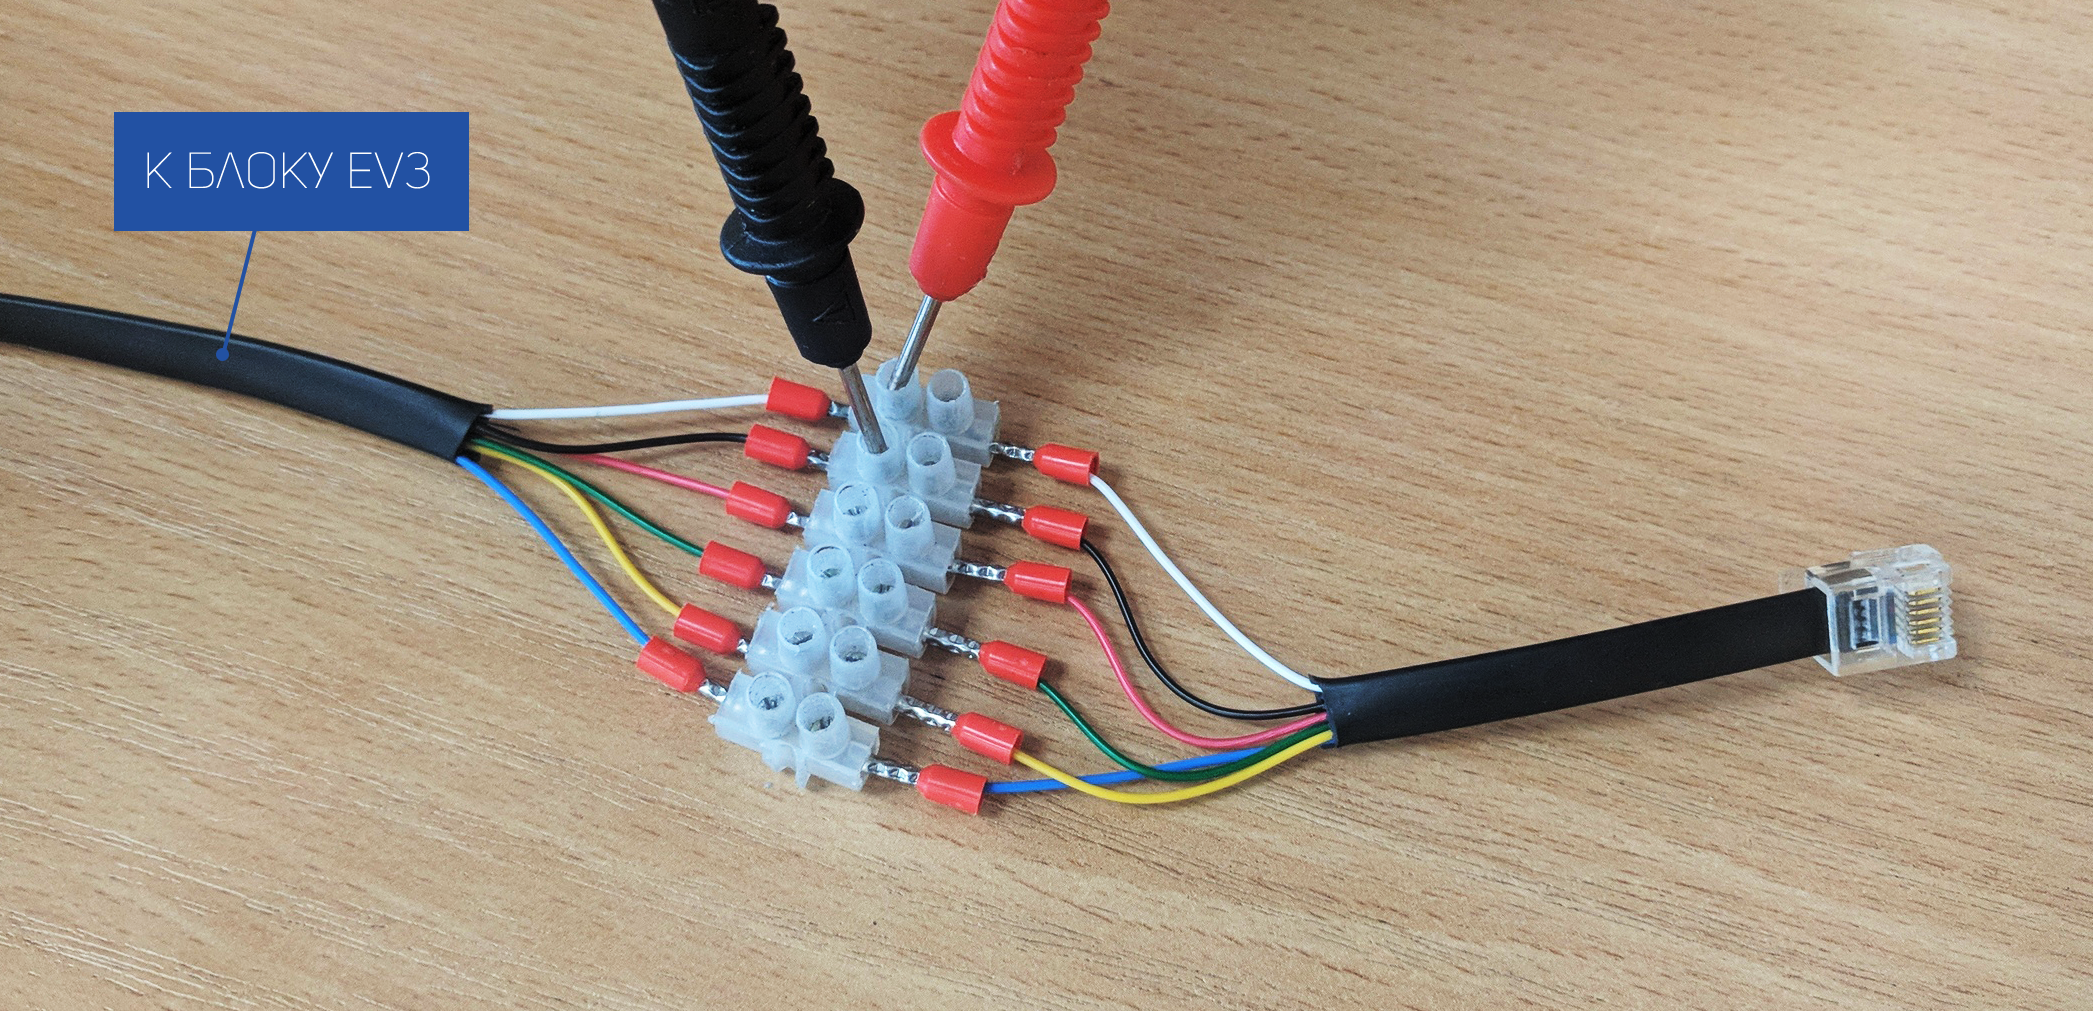
\includegraphics[scale = 0.15]{pics/naprazh_new.png}}
	\caption{Измерение ЭДС.}
	\label{naprazh}
\end{figure}
\item Повторите измерения двух прошлых пунктов при вращении двигателя EV3 в другую сторону.
\item На основании полученных данных постройте в Scilab графики зависимости $U_{ctrl}(I)$ (один график~--- на основании данных, полученных при вращении двигателя в одну сторону, другой~--- на основании данных, полученных при вращении двигателя в другую сторону).
Пример~--- см.~синюю кривую на рис.~\ref{least_squares_method}.
\item В~каждом из случаев аппроксимируйте полученные зависимости линейной функцией $U_{ctrl} = RI$, то есть подберите такое значение коэффициента пропорциональности $R$, при котором график этой функции будет наилучшим образом усреднять полученный результат (пример~--- см.~красную кривую на рис.~\ref{least_squares_method}). Для этого используйте \textit{метод наименьших квадратов}, а точнее формулу
\begin{equation}
	R = \frac{\sum\limits_{j=1}^{10}U_jI_j}{\sum\limits_{j=1}^{10}I^2_j},
\end{equation}
в которой $U_i$, $I_j$~--- результаты $j$-го измерения напряжения и силы тока соответственно.
\begin{figure}[h]
	\center{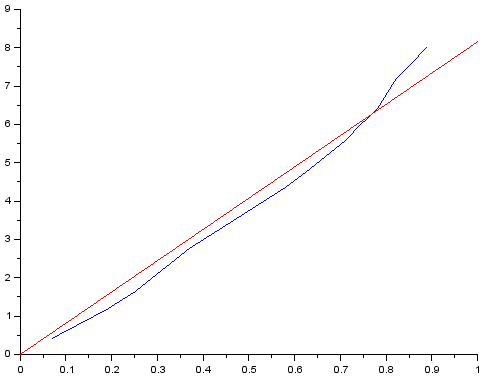
\includegraphics[scale = 0.8]{pics/least_squares_method.png}}
	\caption{Аппроксимация полученных данных.}
	\label{least_squares_method}
\end{figure}
\item Найдите итоговое значение сопротивления как среднее арифметическое от получившихся значений $R$ в каждом из случаев:
\begin{equation}
	R_\textit{итог} = \frac{R_1+R_2}{2},
\end{equation}
\end{enumerate}

\item Определение остальных параметров двигателя
\begin{enumerate}
\item Измерьте массу($m_\textit{р}$) и радиус ($r_\textit{р}$) ротора электродвигателя, находящегося внутри мотора EV3 (рис.~\ref{rotor_in_life}), и рассчитайте его момент инерции по формуле:
\begin{equation}
	J_\textit{эд} = \frac{m_\textit{p}r_\textit{p}^2}2\ldotp
\end{equation}
Умножив полученный результат на квадрат передаточного отношения редуктора, найдите приведенный момент инерции $J$:
\begin{equation}
	J = i^2J_\textit{эд}\ldotp
\end{equation}
\begin{figure}[h]
	\center{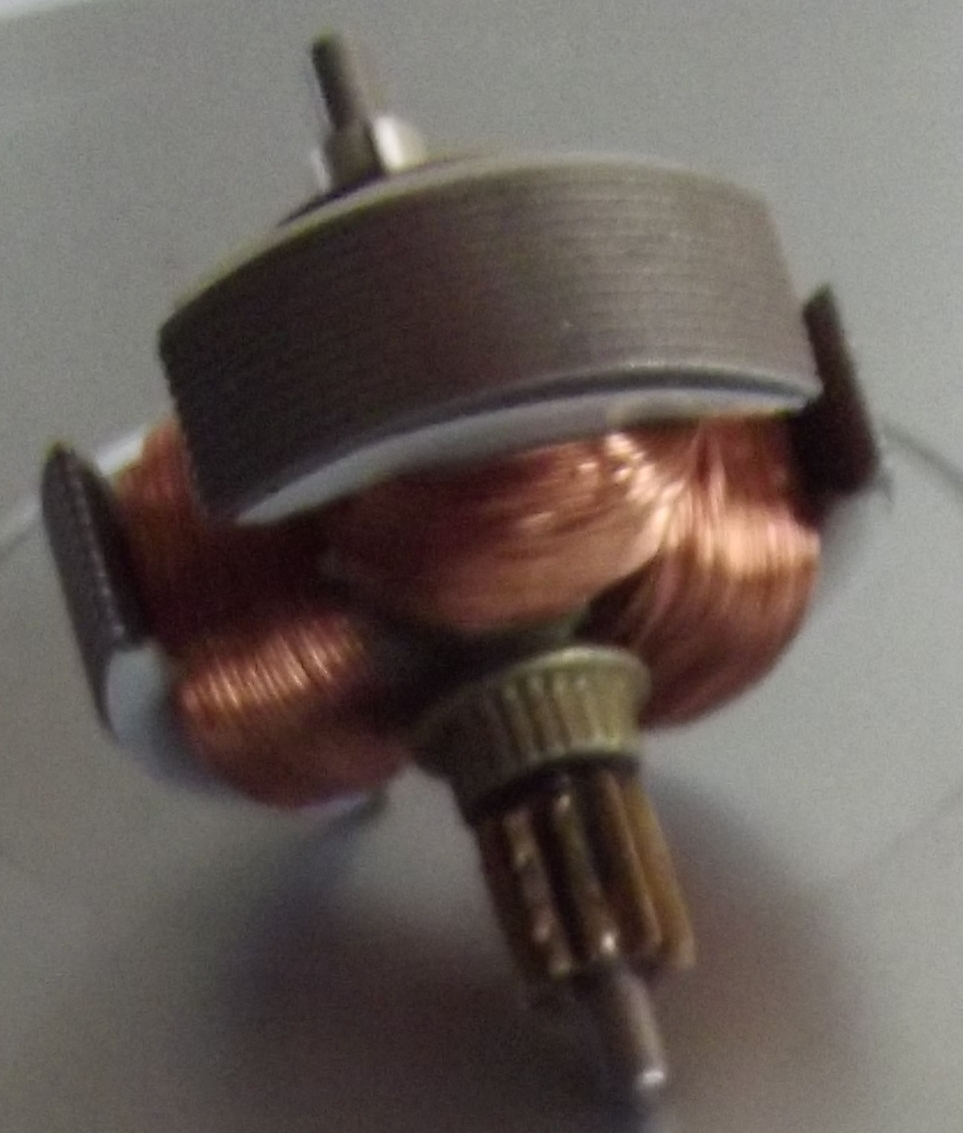
\includegraphics[scale = 0.1]{pics/rotor_in_life.jpg}}
	\caption{Ротор электродвигателя, находящегося внутри мотора EV3.}
	\label{rotor_in_life}
\end{figure}
\item Модифицируйте написанную в первой лабораторной программу так, чтобы она, как и программа из п.~\ref{prog}, запускала двигатель на вращение, поочередно меняя последний аргумент в функции \verb|OnFwd()| c 10 до 100 с шагом 10. При этом свой файл с данными она должна формировать для каждого из запусков двигателя (в итоге должно получиться 10 файлов).
\item Подключите незастопоренный мотор EV3 к кабелю и запустите программу на выполнение. Сохраните полученные в результате ее работы файлы с данными к себе на ПК.
\item Повторите действия прошлого пункта для другого направления вращения вала мотора EV3.
\item Так же, как и в первой лабораторной, обработайте каждый из полученных файлов. На основании достигнутых результатов сформируйте две одностолбцовые (или одностроковые) матрицы\lefteqn,\footnote{Одна матрица будет содержать данные относящиеся к одному направлению вращения вала, вторая~--- к противоположному.} содержащие значения $\omega_{nls}$.  
\item На основании полученных значений скорости и напряжения (последние были получены в п.~\ref{EiiliNaprazh}) подобно тому, как это было сделано при определении сопротивления цепи двигателя, постройте два графика зависимости $\mathcal E_i(\omega)$\footnote{Причины, по которым измеренные напряжения мы принимаем за значения $\mathcal E_i$, указаны в пояснениях к уравнению~\eqref{voltages}.} и аппроксимируйте их функцией $\mathcal E_i=k_e\omega$. Тем самым будут определены два значения для коэффициента $k_e$. За итоговый результат возьмите их среднее значение.

Важно отметить, что поскольку при определении $k_e$ использовались скорости вращения выходного вала мотора EV3, то и полученный коэффициент будет относиться именно к нему. Иными словами, используя ранее введенные обозначения, можно написать $k_e = (r_3/r_1)k_\textit{Д}$.
\item Примите $k_m$ равным $k_e$.
\end{enumerate}
\item Проверка результатов
\begin{enumerate}
\item Постройте схему моделирования процесса разгона ненагруженного двигателя, изображенную на рис.~\ref{struct_sheme_exp}.
Заметим, что она собирает информацию о выходных сигналах, представленных зависимостями $I(t)$ и $\theta(t)$.

Особое внимание при работе с ней обратите на то, что имена переменных, указанных в блоках <<\textsf{To workspace}>> должны различаться, и на то, что значение поля <<Period>> должно иметь для данной схемы довольно маленькое значение, например $0.001$ или меньше. 
В~противном случае графики будут построены грубо, и, как следствие, характерный для графика зависимости $I(t)$ излом может быть прорисован неправильно.  
\begin{figure}[h]
	\center{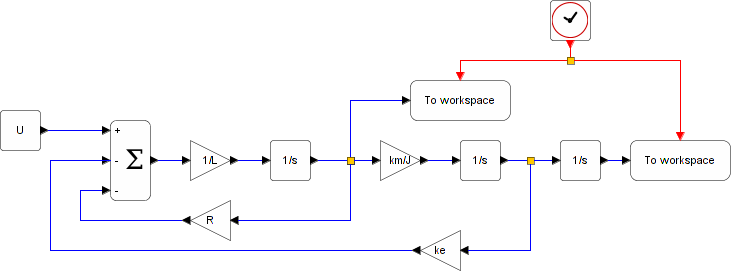
\includegraphics[scale = 0.6]{pics/struct_sheme_exp.png}}
	\caption{Необходимая схема моделирования.}
	\label{struct_sheme_exp}
\end{figure}
\item Аналогично тому, как это было сделано в первой работе, постройте график зависимости $\theta(t)$, соответствующий реальному разгону мотора. Для этого получите такой же, как и в прошлой лабораторной, файл с данными.
\item Промоделируйте собранную схему в Xcos и постройте в том же графическом окне, в котором изображен график функции $\theta(t)$, получающуюся кривую для выходного сигнала $\theta(t)$. Итоговый результат должен быть аналогичен тому, который был достигнут в первой лабораторной (рис.~\ref{second_graph}).
\begin{figure}[h]
	\center{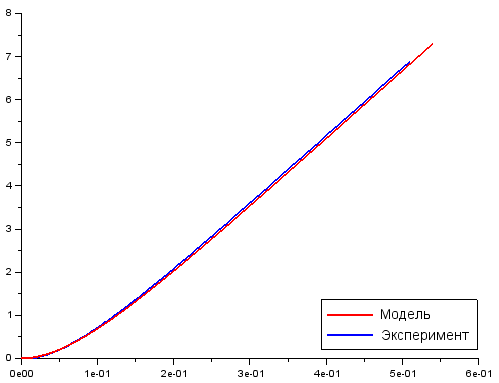
\includegraphics[scale = 0.8]{pics/second_graph.png}}
	\caption{Пример графиков для зависимости $\theta(t)$.}
	\label{second_graph}
\end{figure}
\item В~новом графическом окне постройте график зависимости выходного сигнала $I$ от времени. Полученная кривая должна быть похожа на зеленый график с рис.~\ref{graph_I(t)}.
\end{enumerate}
\item Дополнительные эксперименты со схемой моделирования
\begin{enumerate}
\item Модифицируйте написанную в первой лабораторной программу так, чтобы она подавала на двигатель не постоянное напряжение, а изменяющееся по синусоидальному закону:
\begin{equation}
	U = U_{max}\sin\omega t,
\end{equation}
где $U_{max}$~--- максимальное напряжение питания двигателя, $t$~--- время.
\item Запустите получившуюся программу на той же экспериментальной конструкции (предварительно заменив в последней разрезанный кабель на обычный) на выполнение три раза (при круговой частоте $\omega$, равной $\pi$, $2\pi$ и $3\pi\text{ рад/с}$) и сохраните на свой компьютер все три полученных файла с данными.
\item Для каждого из значений частоты $\omega$ постройте пары графиков, аналогичные представленной на рис.~\ref{graphs_when_sin}. На последнем синий график был построен по данным, записанным EV3 в файл, красный~--- по данным, полученным в результате моделирования схемы, показанной на рис.~\ref{struct_sheme_for_sin}.
\begin{figure}[h]
	\center{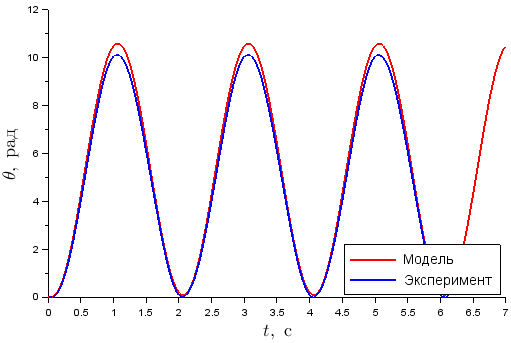
\includegraphics[scale = 0.9]{pics/graphs_when_sin.png}}
	\caption{Необходимая схема моделирования.}
	\label{graphs_when_sin}
\end{figure}
\end{enumerate}
\end{enumerate}

\newpage
\section{Содержание отчета}
\begin{enumerate}
\item Результаты всех измерений, графики и вычисления, предусмотренных(ые) разделом <<Порядок выполнения работы>>, и рассчитанные значения параметров двигателя.
\item Построенные в Xcos блок-схемы (аналогичные представленным на рис.~\ref{struct_sheme_exp} и \ref{struct_sheme_for_sin}).
\item Исходные коды написанных программ, предназначенных для использования с EV3.
\item Выводы о проделанной работе.
\end{enumerate}
\end{document}
